\documentclass[a4paper,14pt]{article}
\usepackage{graphicx}
\usepackage{geometry}
\usepackage{ctex}
\usepackage{pdfpages}
\usepackage[T1]{fontenc}
\usepackage{listings}
\usepackage{xeCJK}  % 使用 xeCJK 宏包支持中文
\setCJKmainfont{宋体}
\setCJKmonofont{宋体}
\setCJKsansfont{宋体}
\usepackage{enumitem}
\usepackage{tabularx}
\usepackage{array}
\usepackage{placeins}
\usepackage{ulem}
\newcolumntype{C}{>{\centering\arraybackslash}X}
\geometry{top=4cm, bottom=4cm, left=2cm, right=2cm}
\setlength{\parindent}{2em}
\usepackage{color}
\usepackage{graphicx}
% 导入代码块
\usepackage{listings}
\usepackage{xcolor}
\usepackage[hidelinks]{hyperref}

\definecolor{codegreen}{rgb}{0,0.6,0}
\definecolor{codegray}{rgb}{0.5,0.5,0.5}
\definecolor{codepurple}{rgb}{0.58,0,0.82}
\definecolor{backcolour}{rgb}{0.95,0.95,0.92}
 
\lstdefinestyle{mystyle}{
    backgroundcolor=\color{backcolour},   
    commentstyle=\color{codegreen},
    keywordstyle=\color{magenta},
    numberstyle=\tiny\color{codegray},
    stringstyle=\color{codepurple},
    basicstyle=\footnotesize,
    breakatwhitespace=false,         
    breaklines=true,             
    captionpos=b,                    
    keepspaces=true,                 
    numbers=left,                    
    numbersep=5pt,                  
    showspaces=false,                
    showstringspaces=false,
    showtabs=false,                  
    tabsize=2
}


\geometry{a4paper, top=2cm, bottom=2cm, left=2cm, right=2cm}



\begin{document}
% 插入PDF第一页作为首页

\includepdf[pages=1]{converted_page.pdf} 
% 插入目录
\tableofcontents
\newpage


\section{实验场景介绍}


图书馆管理系统在大容量藏书和大量读者的环境下,依靠手写记录和人工管理的传统方式已无法满足实际需求。由于手工管理效率低、易出错、数据难以及时更新,无法提供快速、准确的服务。因此,引入基于数据库的图书管理系统显得尤为必要。通过数据库系统,可以实现图书馆藏书的高效管理,涵盖书籍录入、信息查询、借阅、归还等功能,确保系统数据的一致性和准确性,从而提升图书馆的管理效率和服务质量。

系统设计需同时考虑管理员和读者两类用户的需求:
\begin{itemize}
    \item 管理员:管理员在系统中扮演关键角色,负责日常系统管理和维护。其职责包括:
    \begin{itemize}
        \item 新增图书:添加馆藏新书到数据库中。
        \item 删除书籍:清理失效、过期或损坏的书籍,以保证图书馆资源的准确性和整洁性。
        \item 审核借书和还书申请:对读者的借书、还书请求进行审核,确保图书的流通管理。
        \item 信息维护:管理员拥有权限,对图书信息进行增删改查,确保馆藏数据的更新和有效性。
    \end{itemize}
    \item 读者是系统的直接使用者,主要承担图书查询、借阅和归还的任务。其权限受到严格限制,仅能进行特定的操作:
    \begin{itemize}
        \item 查询图书:根据书名、作者等信息查找图书,获取相关详情。
        \item 借阅图书:根据需求从馆藏中借阅图书,记录借书时间。
        \item 归还图书:归还借阅的图书,系统会记录归还时间及状态。
        \item 读者无法修改图书信息,仅能对书籍进行借阅和归还操作,以保证系统数据的一致性和安全性。
    \end{itemize}
\end{itemize}
通过系统设计,能够有效提升图书馆管理效率,减少人力资源的浪费,降低人为错误的发生率,并提升读者的使用体验。同时,系统也能通过权限控制,确保数据安全和操作规范,保障图书管理的科学化、智能化。

\section{数据库设计}

\subsection{概念数据库设计}
\begin{itemize}
    \item 在本项目的概念数据库设计中,我们将主要分为三大部分:图书信息、借阅信息和用户信息。
    \item 图书信息部分包含图书编号、书名、出版社、出版年份、价格、实体编号、馆藏地点、馆藏状态等属性。图书编号用于唯一标识每本书,实体编号用于区分不同版本或实体的图书,以确保同一书名的不同实体能够被准确区分。馆藏地点记录图书在图书馆中的实际存放位置,馆藏状态如“在馆”、“借出”、“损坏”等用于管理图书的流通状态。由于一本书可能由多位作者,因此需要设计一个单独的表来存储作者信息,并通过图书编号与作者进行关联,形成多对多关系。
    \item 用户信息部分使用 Django 内置的 User 和 Group 模型来管理用户信息。我们定义了两种用户组,分别为“读者组”和“管理员组”,并为各自组的用户赋予不同的权限。例如,读者组仅能进行借阅和还书操作,而管理员组则具备图书管理、借阅管理、罚款管理等权限。权限控制的实施确保了不同用户组之间的操作权限的严格划分。
    \item 借阅信息部分主要用于记录每位读者的借阅记录,包括图书编号、读者ID、借阅时间、归还时间、借阅状态和相关罚款ID等。借阅信息表中包含读者ID和图书编号的外键,用于关联用户和图书,而罚款表用于记录因逾期或损坏图书而产生的罚款情况,以确保系统在管理读者借阅行为时能够对逾期或损坏的书籍进行有效追踪和罚款处理。为直观展示数据库设计,我们绘制了 E-R 图,其中包括图书、用户、借阅记录和罚款实体及其之间的关系。
    \item 通过这样的概念数据库设计,我们能够高效管理图书馆藏书,提升图书馆系统的运维效率,为管理员和读者提供更便利的服务。
    \item 设计 E-R 图(Entity-Relationship Diagram):

    \vspace{10pt}
\begin{center}
    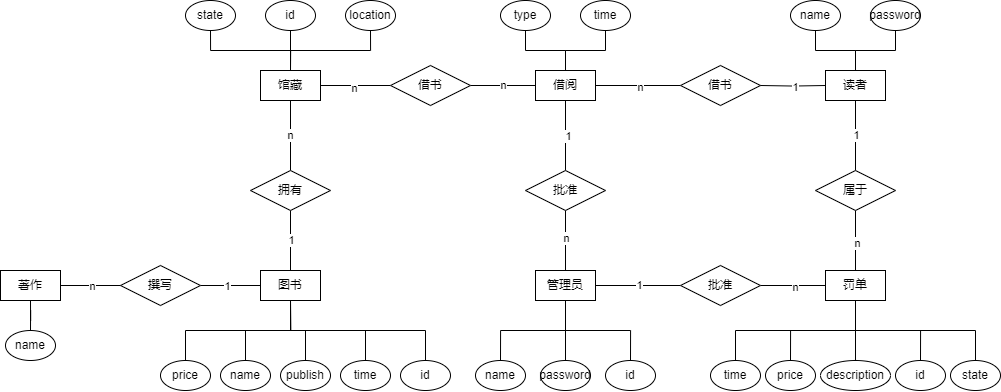
\includegraphics[width=\linewidth]{images/ERphoto.png}\end{center}
\vspace{5pt}


    \item 各实体及其属性(其中主键用下划线表示,外键用双下划线表示):
    \begin{itemize}
        \item 图书信息表:\underline{图书编号},书名,出版社,出版时间,价格;
        \item 馆藏信息表:\underline{馆藏编号},\uuline{图书编号},馆藏地点,状态;
        \item 著作表:\underline{图书编号},\underline{作者};
        \item 借阅信息表:\underline{借书编号},\uuline{读者编号},\uuline{管理员编号},\uuline{馆藏编号},时间,操作类型;
        \item 读者信息表:\underline{读者编号},姓名,密码;
        \item 管理员信息表:\underline{管理员编号},姓名,密码;
        \item 罚款信息表:\underline{罚款编号},\uuline{管理员编号},\uuline{读者编号},金额,时间,描述,状态。
        
    \end{itemize}
\end{itemize}

\subsection{逻辑数据库设计}

\begin{table}[htbp]
    \centering
    \caption{图书信息表}
    \begin{tabularx}{\textwidth}{|C|C|C|C|C|}
    \hline
    字段 & 类型 & 主键/外键 & 取值 & 备注 \\
    \hline
    ID & INTEGER & 主键 &  & 自增主键 \\
    \hline
    NAME & VARCHAR(150) &  &  & 书籍名 \\
    \hline
    PUBLISH & VARCHAR(150) &  &  & 出版社 \\
    \hline
    TIME & INTEGER &  & 正整数 & 出版年份 \\
    \hline
    PRICE & DECIMAL &  & 正数 & 书籍价格 \\
    \hline
    \end{tabularx}
\end{table}

    \begin{table}[htbp]
    \centering
    \caption{馆藏信息表}
    \begin{tabularx}{\textwidth}{|C|C|C|C|C|}
        \hline
        字段 & 类型 & 主键/外键 & 取值 & 备注 \\
        \hline
        ID & INTEGER & 主键 &  & 自增主键 \\
        \hline
        BOOK\_ID & INTEGER & 外键 &  & 书籍外键 \\
        \hline
        LOCATION & VARCHAR(150) &  &  & 馆藏地点 \\
        \hline
        STATE & SMALLINT &  & 0,1,2 & 0借出,1在馆,2损毁 \\
        \hline
        \end{tabularx}
\end{table}

    \begin{table}[htbp]
    \centering
    \caption{著作表}
    \begin{tabularx}{\textwidth}{|C|C|C|C|C|}
        \hline
        字段 & 类型 & 主键/外键 & 取值 & 备注 \\
        \hline
        ID & INTEGER & 主键 &  & 自增主键 \\
        \hline
        BOOK\_ID & INTEGER &  &  & 书籍外键(与作者名的组合唯一) \\
        \hline
        WRITER & VARCHAR(150) &  &  & 作者名 \\
        \hline
        \end{tabularx}
\end{table}

\begin{table}[htbp]
    \centering
    \caption{用户表}
    \begin{tabularx}{\textwidth}{|C|C|C|C|C|}
    \hline
    字段 & 类型 & 主键/外键 & 取值 & 备注 \\
    \hline
    ID & INTEGER & 主键 &  & 自增主键 \\
    \hline
    USERNAME & VARCHAR(150) &  &  & 用户名 \\
    \hline
    PASSWORD & VARCHAR(128) &  &  & 密码 \\
    \hline
    FIRSTNAME & VARCHAR(30) &  &  & 名 \\
    \hline
    LASTNAME & VARCHAR(150) &  &  & 姓 \\
    \hline
    EMAIL & VARCHAR(254) &  &  & 邮箱 \\
    \hline
    \end{tabularx}
\end{table}

\begin{table}[htbp]
    \centering
    \caption{借阅信息表}
    \begin{tabularx}{\textwidth}{|C|C|C|C|C|}
    \hline
    字段 & 类型 & 主键/外键 & 取值 & 备注 \\
    \hline
    ID & INTEGER & 主键 &  & 自增主键 \\
    \hline
    STORE\_ID & INTEGER & 外键 &  & 馆藏外键 \\
    \hline
    READER\_ID & INTEGER & 外键 &  & 用户外键 \\
    \hline
    TIME & DATETIME &  &  & 记录时间 \\
    \hline
    TYPE & SMALLINT &  & 0,1,2 & 借出/归还/续借 \\
    \hline
    \end{tabularx}
\end{table}

    \begin{table}[htbp]
    \centering
    \caption{罚单表}
    \begin{tabularx}{\textwidth}{|C|C|C|C|C|}
        \hline
        字段 & 类型 & 主键/外键 & 取值 & 备注 \\
        \hline
        ID & INTEGER & 主键 &  & 自增主键 \\
        \hline
        READER\_ID & INTEGER & 外键 &  & 用户外键 \\
        \hline
        PRICE & DECIMAL &  &  & 金额 \\
        \hline
        DESCRIPTION & VARCHAR(150) &  &  & 描述 \\
        \hline
        TIME & DATETIME &  &  & 时间 \\
        \hline
        STATE & SMALLINT &  & 0,1 & 未完成/完成 \\
        \hline
        \end{tabularx}
\end{table}
\FloatBarrier
\section{系统功能介绍}
系统使用Python语言实现,采用B-S架构,使用了Python的Django框架,数据库使用了sqlite3,界面设计使用了BootStrap库以及相应的设计器设计而成,还使用了一些js辅助实现。
Django数据库设计主要在应用目录下的models.py,定义了每张表的内容。
url.py主要负责url地址到视图函数的映射;
views.py主要是具体的视图函数,也就是功能函数。

\subsection{用户登录与登出} 在图书管理系统中,用户认证是系统运行的核心功能之一,确保系统能够有效区分不同权限的用户并提供个性化的服务。基于 Django 框架的内置用户认证功能,系统实现了完善的登录与登出模块。

用户通过登录页面输入用户名和密码,系统会调用 Django 提供的 authenticate\(\) 方法验证用户凭据的正确性。在认证成功后,系统会根据用户所属组(读者或管理员)进行角色区分,并通过 login\(\) 方法记录用户的登录状态,同时跳转到对应的首页。管理员将进入后台管理页面,而普通读者则跳转到读者界面。

当用户选择登出时,系统调用 logout\(\) 方法清除用户的登录会话,并将其重定向到登录页面,确保用户在退出时数据安全。为增强用户体验,登录界面还提供了多种错误提示,如用户名不存在、密码错误或用户已被禁用。此外,为提升系统的安全性,登录模块引入了防爆破机制,限制连续错误登录尝试的次数,避免恶意攻击。

\subsection{数据库查询} 
图书馆系统中的数据库查询功能是管理员和读者获取图书信息的重要途径。系统提供了多种查询条件,包括书名、作者、出版年份和馆藏地点等。这些查询方式分为精确查询和模糊查询:当用户准确知晓图书的特定信息时,可进行精确查询来快速定位图书;若用户只记得部分信息,利用模糊查询能找到包含该部分信息的所有相关图书。

系统基于 SQL 语句实现查询功能。当用户在搜索框输入关键字后,系统会在后台构建相应的 SQL 查询语句并与数据库交互:根据用户输入的关键字和所选查询字段(如书名、作者等)来构建 SQL 查询语句。例如,若用户在书名字段输入 “数据库”,系统会判断是精确查询还是模糊查询,进而生成如上述示例的查询语句。构建好查询语句后,将其发送到后端数据库sqlite3进行查询操作,数据库执行后将符合条件的图书记录返回给系统。

查询结果以表格形式呈现于页面上,每行对应一本书的记录,包含书籍名称、出版社、出版时间、状态等信息。其中,书名以超链接形式存在,点击可查看书籍详细内容;对于有多个作者的书籍,系统可通过在 SQL 查询语句中使用合适的连接和分组操作来获取并展示所有作者信息,保证信息全面直观。

管理员在查询结果页面可进行更多操作,可直接对书籍记录进行修改或删除操作。修改操作通过点击相应按钮进入编辑页面,在后台通过 SQL 的UPDATE语句实现;删除操作可直接从数据库中删除记录,通过DELETE语句实现。

当查询无结果时,系统通过判断查询返回的记录集为空,友好地提示 “未找到相关图书”,避免用户困惑,提升用户体验。对于一些复杂的查询业务,如查询借阅书籍数量超过平均借阅数量的读者信息或查询所有逾期未还书籍的读者姓名、书籍名称及相应罚款信息等,都通过精心编写 SQL 语句来实现。通过这种方式,图书馆系统的数据库查询功能不仅能满足基本查询需求,还能处理复杂业务逻辑查询,为图书馆管理和运营提供有力的数据支持。


\subsection{数据库修改} 管理员在日常工作中,可能需要对已有图书信息进行调整,如修正错误的数据或更新图书的馆藏状态。数据库修改功能旨在提供安全、便捷的编辑操作。

系统通过 Django 的表单组件(ModelForm)实现数据的接收和验证。管理员点击某本书籍的“编辑”按钮后,系统将当前记录的信息加载到表单中供管理员修改。用户提交修改后,系统会对新数据进行校验,确保其符合数据库约束条件。例如,出版年份需为有效的正整数,价格字段必须为正数等。若验证通过,修改将被保存至数据库,同时在页面显示“修改成功”的提示;若验证失败,系统会将错误信息反馈给用户,要求重新填写。

为确保数据的一致性和完整性,系统设计了事务机制:任何异常操作都会触发回滚,避免不完整数据被写入数据库。此外,修改功能限定仅管理员可访问,普通用户尝试访问时会被系统拦截,重定向至权限不足页面。

\subsection{数据库添加} 新书录入是图书馆的重要工作。为确保录入操作的高效性和准确性,系统设计了管理员专用的书籍添加模块。

当管理员进入新书录入页面时,系统会加载一个空表单,表单包括书籍名称、作者、出版时间、价格、馆藏地点等字段。管理员填写完整信息后提交,系统通过表单验证数据的合法性。例如,书名和作者字段不能为空,价格字段需为正数,出版时间必须为合理的年份范围。若验证通过,系统调用 save\(\) 方法将新书信息存入数据库,并在页面显示成功提示。

为防止重复录入,系统会在提交数据前检查是否存在相同的图书记录(如书名和作者组合相同)。若发现重复数据,系统会中止录入并提示管理员检查输入内容。新书录入成功后,管理员可直接从提示页面跳转至书籍详情页或继续录入其他图书,极大提升了工作效率。

\subsection{数据库删除} 删除功能主要用于清理无用或错误的图书记录。管理员可通过书籍列表中的删除按钮触发删除操作,系统会根据书籍的唯一 ID 定位对应的记录并尝试删除。

在删除前,系统会提示管理员确认操作,以避免误删数据。如果管理员确认删除,系统将调用 delete\(\) 方法执行操作,并将结果返回给用户,提示“删除成功”或“删除失败”。删除操作受权限控制,仅授权管理员可执行,普通用户尝试访问删除功能将被拒绝。

为避免数据丢失,系统设计了软删除机制:删除操作不会直接清理数据库中的记录,而是将状态字段标记为“已删除”,从而保留历史记录。这种设计便于管理员在需要时恢复已删除的数据,同时避免因误操作造成的数据不可恢复问题。

\subsection{对图书的操作} 借书、还书和续借是系统的核心功能模块,旨在实现图书流通的高效管理。

\subsubsection{借书功能}
用户在界面中选择目标书籍后,系统通过提交的藏书 ID 和用户 ID 验证用户权限及书籍状态。若书籍在馆且无其他限制条件(如逾期罚款未缴清),系统生成借阅记录,并更新书籍的馆藏状态为“借出”。同时,系统会记录借阅时间、借阅者信息等,并为用户提供借阅成功的提示。

\subsubsection{还书功能}
用户选择还书后,系统会根据提交的藏书 ID 查找借阅记录,验证书籍当前状态是否为“借出”。还书操作完成后,系统更新馆藏状态为“在馆”,并根据还书时间计算是否产生逾期罚款。若存在罚款情况,系统会生成罚单记录并通知用户。

\subsubsection{续借功能}
续借操作适用于用户需要延长借阅时间的场景。用户在借阅到期前发起续借请求,系统检查图书是否符合续借条件(如本人没有罚单、当前借阅次数未超限制)。若满足条件,系统更新借阅记录并延长借阅时间;否则提示续借失败。

通过这些功能模块,系统能够实现对图书流通的全生命周期管理,同时为用户提供便捷的操作体验和清晰的反馈。



\section{核心代码示例}

\subsection{查询每个读者的借阅记录,包括读者姓名、借阅书籍名称、借阅时间}
\begin{lstlisting}[language=sql,breaklines=true]
SELECT 
    r.reader_name,
    b.book_name,
    li.loan_time
FROM 
    LoanInfo li
JOIN 
    ReaderInfo r ON li.reader_id = r.reader_id
JOIN 
    StoreInfo si ON li.store_id = si.store_id
JOIN 
    BookInfo b ON si.book_id = b.book_id;
\end{lstlisting}

查询逻辑:从 LoanInfo 表开始,使用 JOIN 操作将 LoanInfo 表与 ReaderInfo 表连接起来,连接条件是 li.reader\_id = r.reader\_id,获取每个借阅记录对应的读者信息;将结果集与 StoreInfo 表连接,连接条件是 li.store\_id = si.store\_id,得到借阅的馆藏信息;再将结果集与 BookInfo 表连接,连接条件是 si.book\_id = b.book\_id,获取借阅书籍的详细信息,最终选择读者姓名(r.reader\_name)、书籍名称(b.book\_name)和借阅时间(li.loan\_time)作为查询结果。


\subsection{查询有未处理罚单的读者的借阅记录,包括读者姓名、借阅书籍名称、借阅时间}
\begin{lstlisting}[language=sql, breaklines=true]
SELECT 
    r.reader_name,
    b.book_name,
    li.loan_time
FROM 
    LoanInfo li
JOIN 
    ReaderInfo r ON li.reader_id = r.reader_id
JOIN 
    StoreInfo si ON li.store_id = si.store_id
JOIN 
    BookInfo b ON si.book_id = b.book_id
WHERE 
    r.reader_id IN (
        SELECT 
            reader_id 
        FROM 
            FineInfo 
        WHERE 
            fine_status = 'unprocessed'
    );
\end{lstlisting}

查询逻辑:首先构建一个子查询,从 FineInfo 表中筛选出 fine\_status 为 unprocessed的记录,提取这些记录中的 reader\_id,然后进行主查询,与前面查询每个读者借阅记录的方式类似,从 LoanInfo 表开始,通过 JOIN 操作依次连接 ReaderInfo、StoreInfo 和 BookInfo 表,最后 WHERE 子句过滤出 reader\_id 在子查询结果集中的记录,即有未处理罚单的读者的借阅记录,并选择读者姓名、书籍名称和借阅时间作为查询结果。

\subsection{查询借阅过特定书籍的读者的未处理罚单信息}
\begin{lstlisting}[language=sql, breaklines=true]
SELECT*FROM 
    FineInfo
WHERE 
    reader_id IN (
        SELECT 
            reader_id 
        FROM 
            LoanInfo 
        WHERE 
            store_id IN (
                SELECT 
                    store_id 
                FROM 
                    StoreInfo 
                WHERE 
                    book_id = <specific_book_id>
            )
    )
    AND fine_status = 'unprocessed';
\end{lstlisting}

查询逻辑:最内层子查询从 StoreInfo 表中筛选出 book\_id 等于 <book\_id>的记录,提取这些记录中的 store\_id;中间子查询从 LoanInfo 表中筛选出 store\_id 在最内层子查询结果集中的记录,提取这些记录中的 reader\_id,即借阅过特定书籍的读者的 reader\_id;主查询从 FineInfo 表中筛选出 reader\_id 在中间子查询结果集中且 fine\_status 为 unprocessed的记录,即借阅过特定书籍且有未处理罚单的读者的罚款信息。


\subsection{查询每个管理员处理的借阅记录和相关书籍信息,只显示状态为借出的书籍}
\begin{lstlisting}[language=sql, breaklines=true]
SELECT 
    a.admin_name,
    li.loan_time,
    b.book_name,
    si.store_status
FROM 
    LoanInfo li
JOIN 
    AdminInfo a ON li.admin_id = a.admin_id
JOIN 
    StoreInfo si ON li.store_id = si.store_id
JOIN 
    BookInfo b ON si.book_id = b.book_id
WHERE 
    si.store_status = 'borrowed';
\end{lstlisting}

查询逻辑:从 LoanInfo 表开始,通过 JOIN 操作将其与 AdminInfo 表连接,连接条件是 li.admin\_id = a.admin\_id,以获取处理借阅记录的管理员信息;将结果集与 StoreInfo 表连接,连接条件是 li.store\_id = si.store\_id,得到借阅的馆藏信息;将结果集与 BookInfo 表连接,连接条件是 si.book\_id = b.book\_id,获取书籍信息;最后用 WHERE 子句过滤出 si.store\_status 为 borrowed的记录,即只显示状态为借出的书籍的相关信息。


\subsection{查询借阅书籍数量超过平均借阅数量的读者信息}
\begin{lstlisting}[language=sql, breaklines=true]
SELECT*FROM 
    ReaderInfo
WHERE 
    reader_id IN (
        SELECT 
            reader_id 
        FROM (
            SELECT 
                reader_id, 
                COUNT(*) AS total_loans
            FROM 
                LoanInfo
            GROUP BY 
                reader_id
        ) AS sub
        WHERE 
            total_loans > (
                SELECT 
                    AVG(total_loans)
                FROM (
                    SELECT 
                        COUNT(*) AS total_loans
                    FROM 
                        LoanInfo
                    GROUP BY 
                        reader_id
                ) AS sub_avg
            )
    );
\end{lstlisting}

查询逻辑:在最内层子查询中从 LoanInfo 表按 reader\_id 进行分组,并统计每个读者的借阅次数,将结果命名为 total\_loans,得到每个读者的借阅书籍数量;中间子查询从上述结果中筛选出 total\_loans 大于平均借阅数量的记录,提取这些记录中的 reader\_id。平均借阅数量通过另一个子查询sub\_avg计算得出,子查询从 LoanInfo 表按 reader\_id 分组统计借阅次数,然后使用 AVG 函数计算平均值。主查询从 ReaderInfo 表中筛选出 reader\_id 在中间子查询结果集中的记录,即借阅书籍数量超过平均借阅数量的读者信息。

\subsection{查询所有逾期未还书籍的读者姓名、书籍名称以及相应的罚款信息}
\begin{lstlisting}[language=python, breaklines=true]
SELECT 
    r.reader_name,
    b.book_name,
    fi.fine_amount,
    fi.fine_description
FROM 
    LoanInfo li
JOIN 
    ReaderInfo r ON li.reader_id = r.reader_id
JOIN 
    StoreInfo si ON li.store_id = si.store_id
JOIN 
    BookInfo b ON si.book_id = b.book_id
LEFT JOIN 
    FineInfo fi ON li.reader_id = fi.reader_id AND si.store_id = (
        SELECT 
            store_id 
        FROM 
            LoanInfo 
        WHERE 
            loan_type = 'borrow' 
            AND loan_status = 'unreturned' 
            AND DATEDIFF(CURDATE(), loan_time) > 30
    )
WHERE 
    li.loan_type = 'borrow' 
    AND li.loan_status = 'unreturned' 
    AND DATEDIFF(CURDATE(), li.loan_time) > 30;
\end{lstlisting}

查询逻辑:从 LoanInfo 表开始,通过 JOIN 操作依次与 ReaderInfo、StoreInfo 和 BookInfo 表连接,以获取读者姓名、书籍名称等基本信息,用 LEFT JOIN 将 FineInfo 表连接到前面的结果集,连接条件是 li.reader\_id = fi.reader\_id 且 si.store\_id 等于一个子查询的结果。该子查询从 LoanInfo 表中筛选出 loan\_type 为 borrow、loan\_status 为 unreturned且逾期天数大于 30 天的记录的 store\_id。最后用 WHERE 子句筛选出 li.loan\_type 为 borrow、li.loan\_status 为 unreturned 且逾期天数大于 30 天的记录,即所有逾期未还书籍的相关信息,包括读者姓名、书籍名称以及相应的罚款信息。

\section{效果展现}
\subsection{首页}
\subsubsection{登录与登出}
在终端注册账户,使用命令注册新账户:
\begin{lstlisting}
    python manage.py createsuperuser
\end{lstlisting}


\begin{center}
    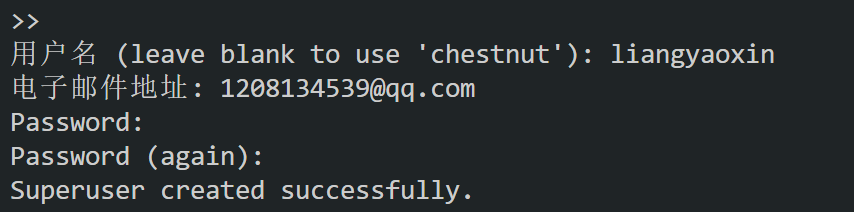
\includegraphics[width=0.3\linewidth]{images/login.png}\end{center}



分别注册好管理员账户和用户账户,即可登录网页。还未登录时,网页显示首页(对东南大学图书馆的介绍):

\vspace{10pt}
\begin{center}
    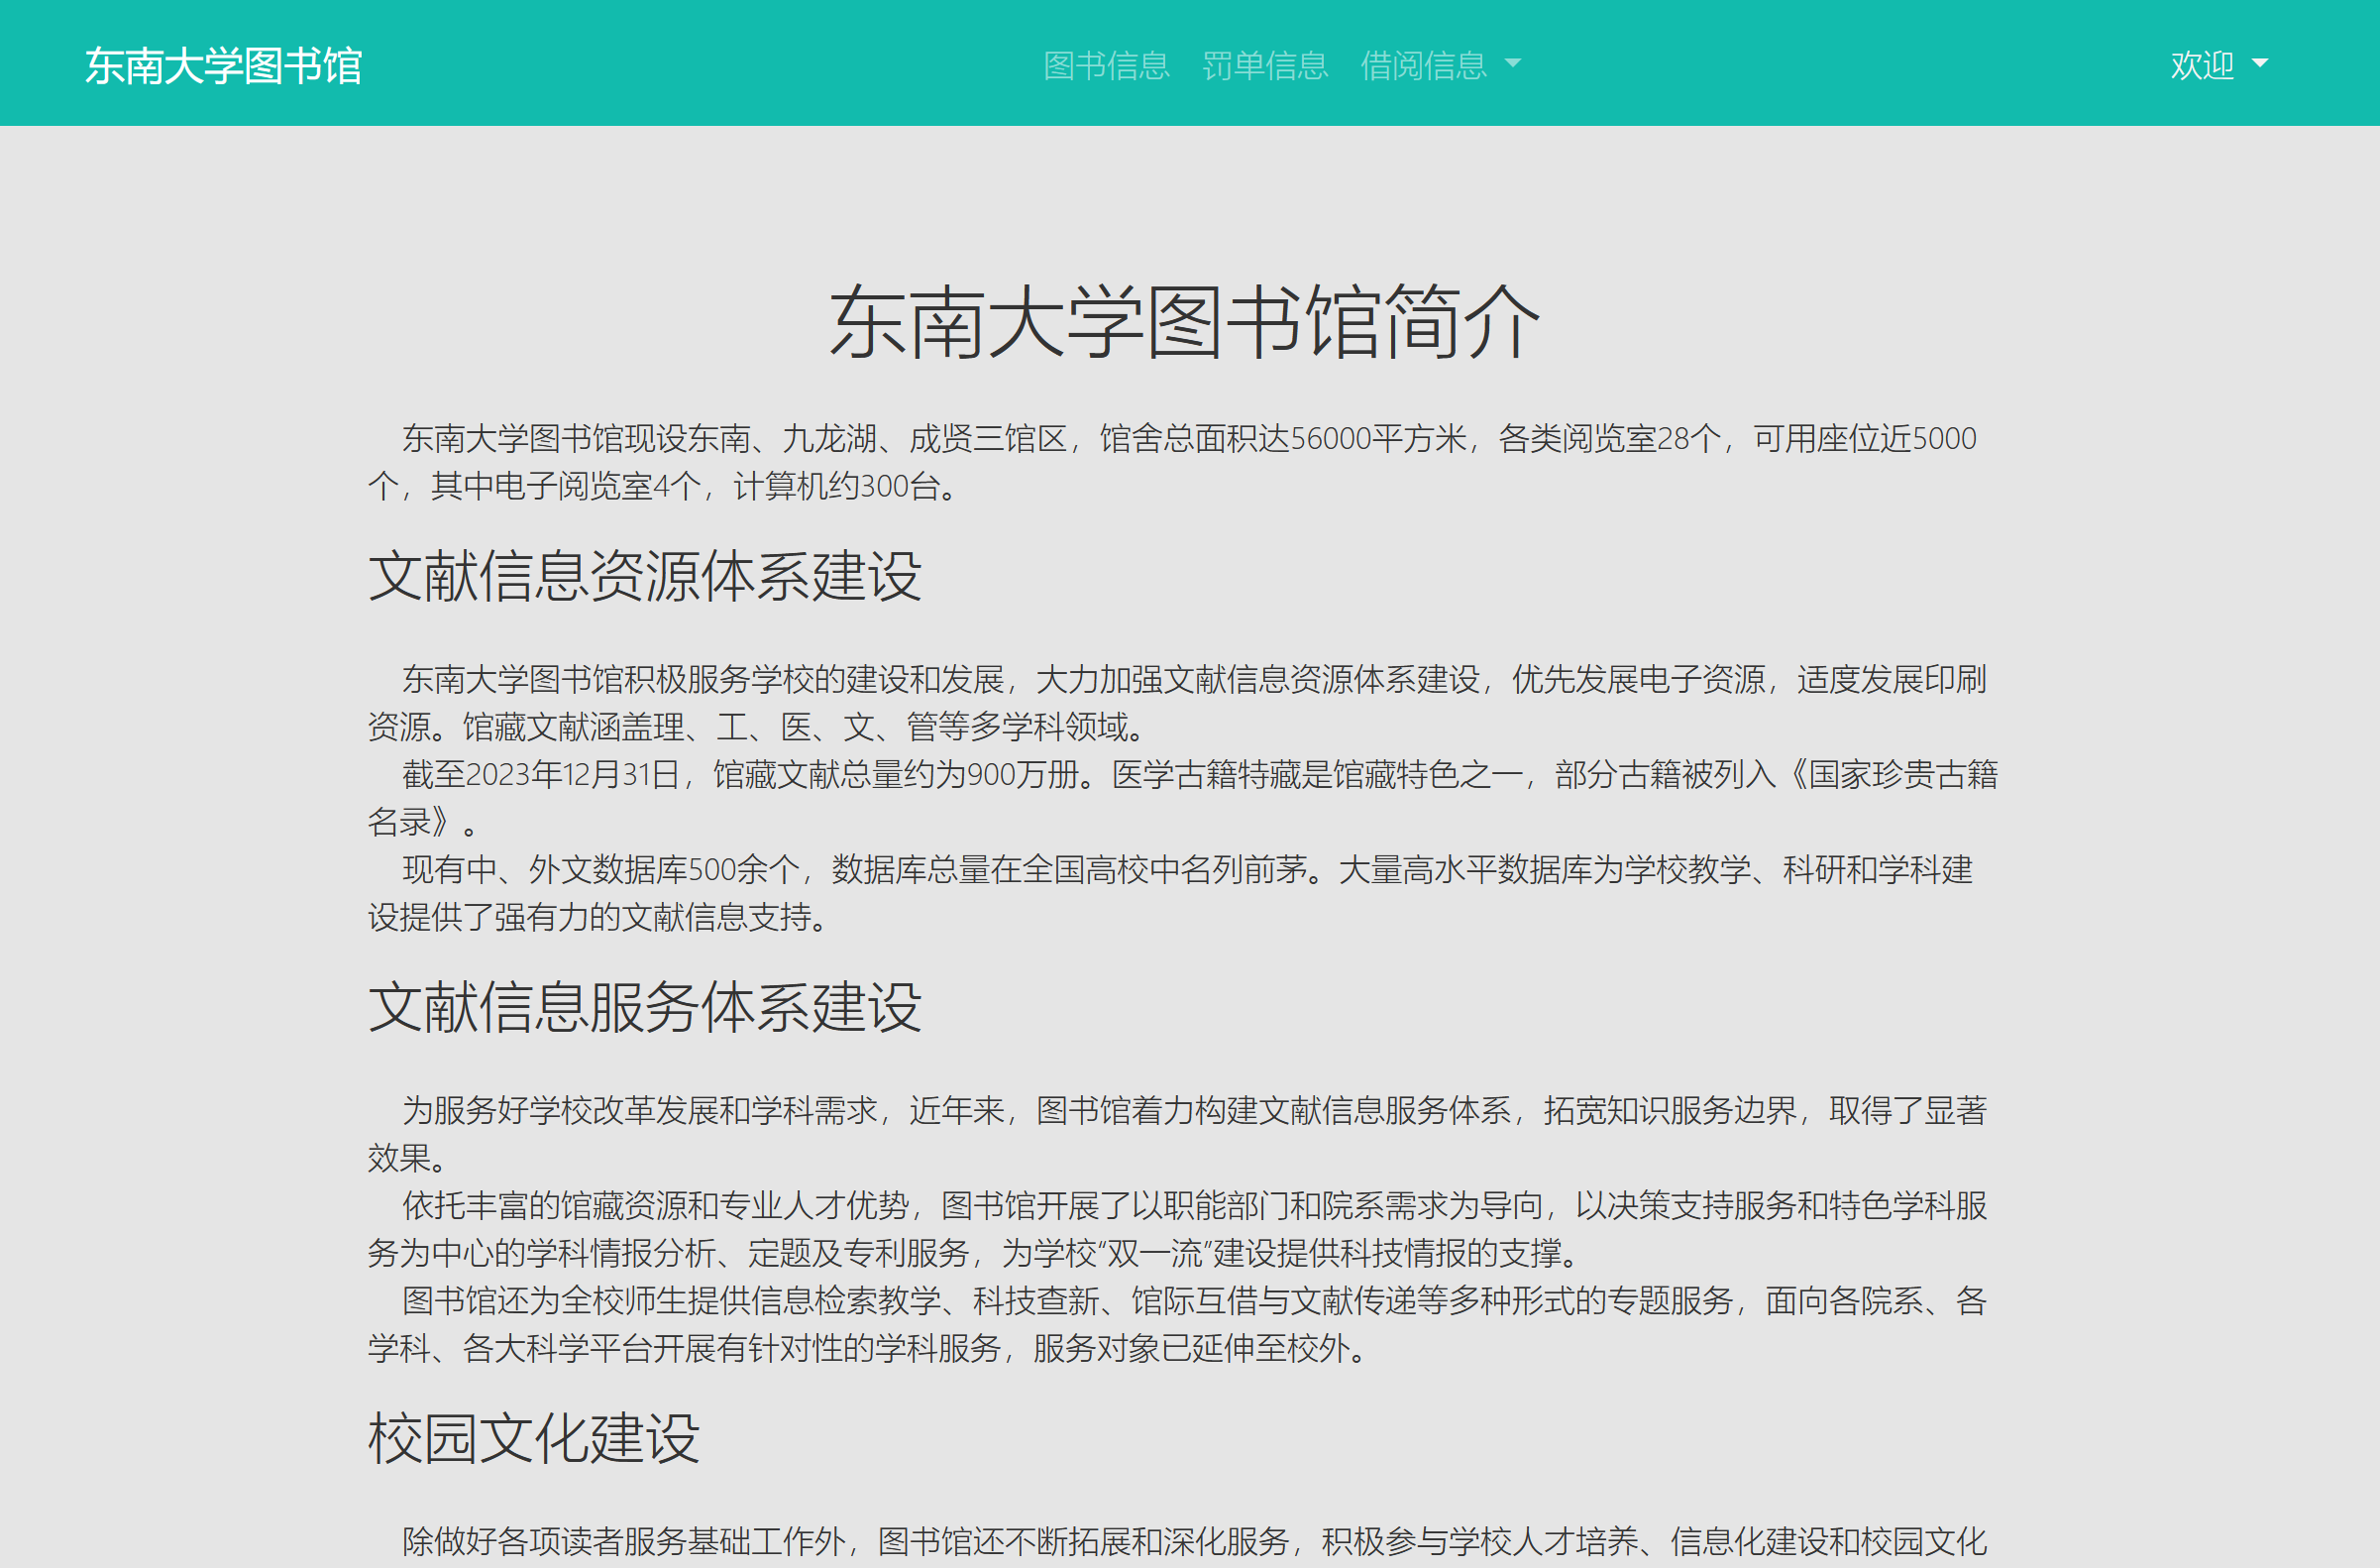
\includegraphics[width=0.8\linewidth]{images/index1.png}\end{center}
\vspace{5pt}


点击右上角进行登录,输入账户密码,输入错误时网站会提示错误,输入正确时会跳转到用户的页面或管理员的页面。

\vspace{10pt}
\begin{center}
    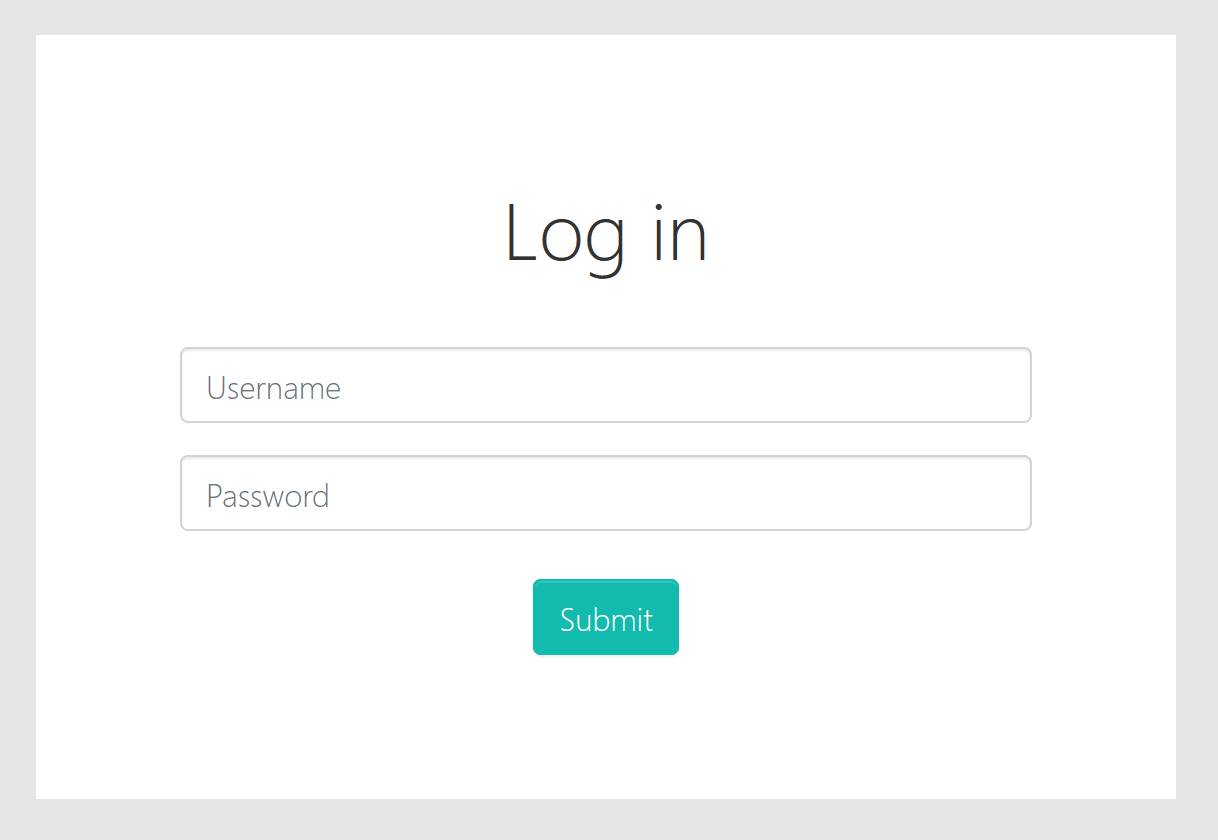
\includegraphics[width=0.3\linewidth]{images/login2.png}\end{center}
\vspace{5pt}


成功进入用户页面,会看到右上角提示登陆用户名。

\subsection{管理员页面}
\subsubsection{查询操作}
在“搜索图书”页面输入书籍的名称、作者名字、借阅等信息进行查询,可以显示匹配到的书籍信息,点击书名可以查看书籍的详细信息并管理书籍信息、作者信息、馆藏信息;点击删除可以对书籍进行删除操作:

\vspace{10pt}
\begin{center}
    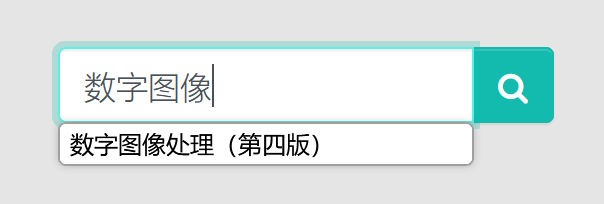
\includegraphics[width=0.3\linewidth]{images/chaxun1.png}\end{center}

\begin{center}
    
\includegraphics[width=0.3\linewidth]{images/chaxun2.png}\end{center}

\begin{center}
    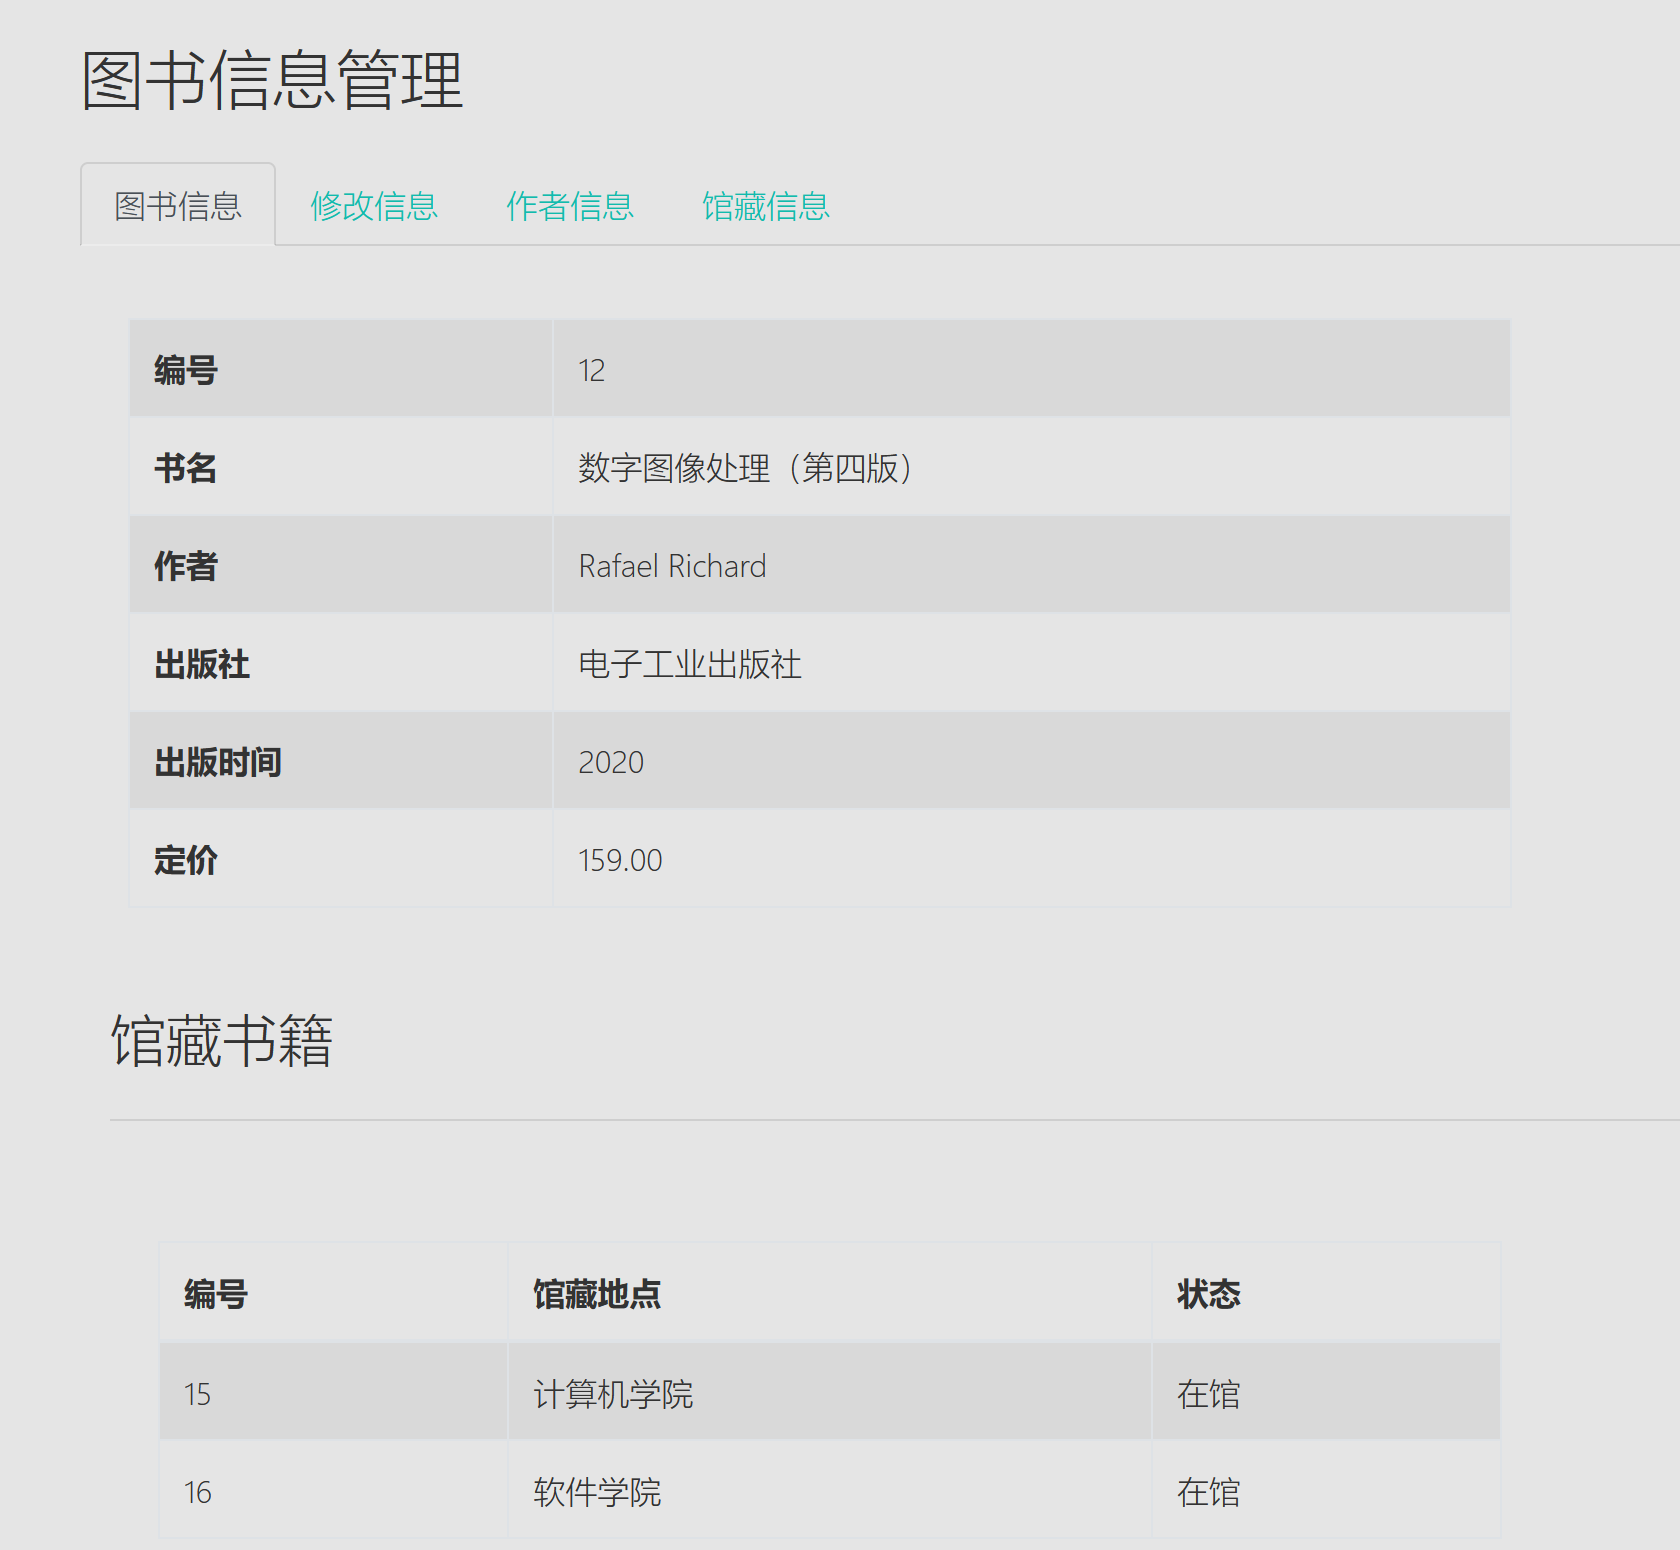
\includegraphics[width=0.7\linewidth]{images/chaxun3.png}\end{center}
\vspace{5pt}

同时,可以查询借阅过特定书籍的读者的未处理罚单信息;在super管理员处可以进行每个管理员处理的借阅记录和相关书籍的信息,只显示状态为借出的书籍。在罚单页面也可以进行输入书籍的名称、作者名字、借阅等信息之后的查询操作,页面效果类似,可以返回读者姓名、书籍名称、借阅时间信息。
在搜索图书页面点击“最佳借阅”可以跳转至查询借阅书籍数目超过平均借阅数量的读者的信息:

\vspace{10pt}
\begin{center}
    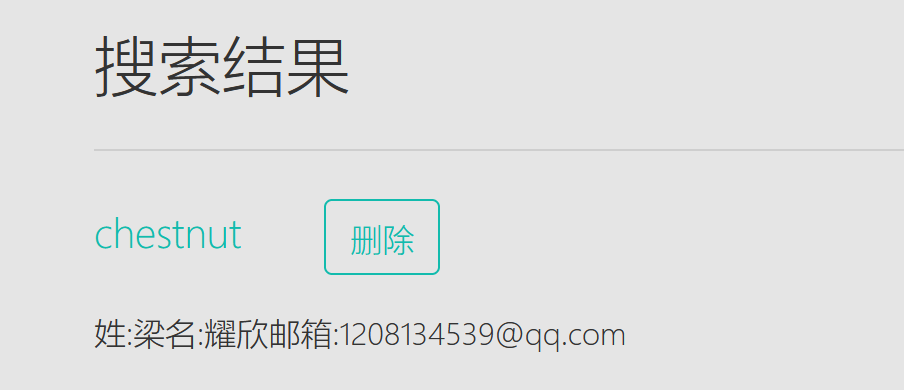
\includegraphics[width=0.4\linewidth]{images/222.png}\end{center}
\vspace{5pt}

查询有逾期未归还的读者信息和书籍名称和罚款信息,在罚单页面、借阅页面、还书页面都可以进行查询操作,点击确定后会跳转到查询结果页面:

\vspace{10pt}
\begin{center}
    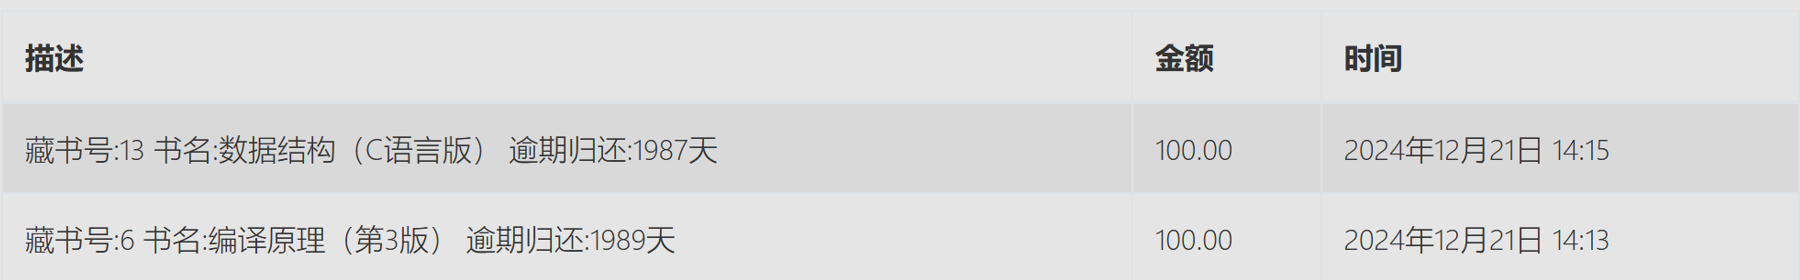
\includegraphics[width=0.7\linewidth]{images/111.png}\end{center}
\vspace{5pt}

\subsubsection{删除操作}
在书籍信息管理页面可以对作者、馆藏分别进行删除操作;在书籍查询页面可以对书籍进行删除操作,成功后会提示删除成功并把这条记录从数据库中删除:

\vspace{10pt}
\begin{center}
    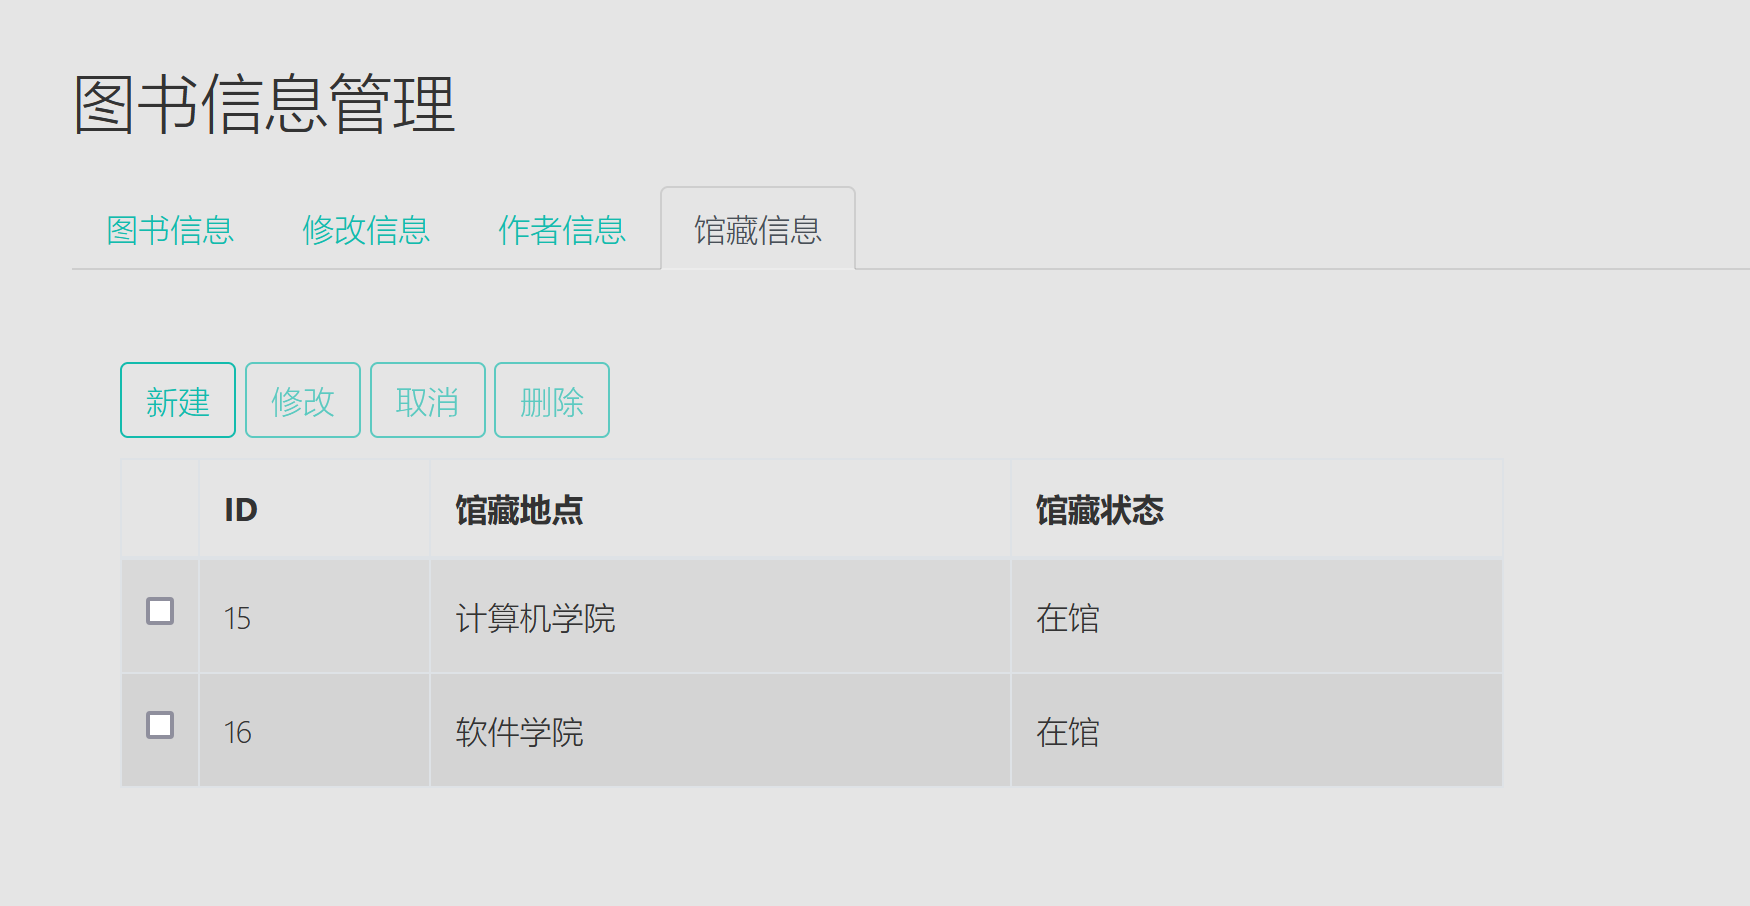
\includegraphics[width=0.7\linewidth]{images/shanchu1.png}\end{center}
\vspace{5pt}


\vspace{10pt}
\begin{center}
    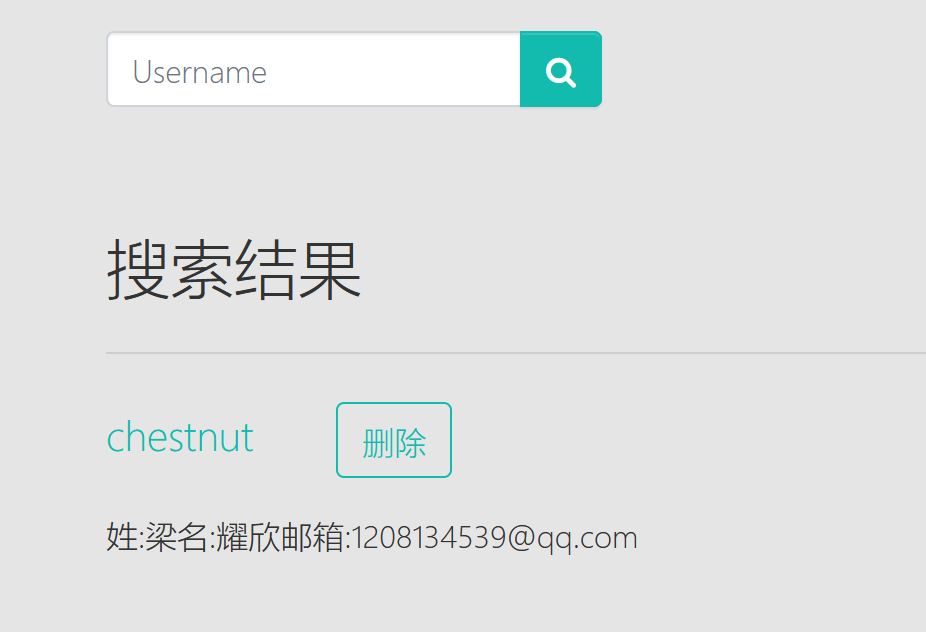
\includegraphics[width=0.4\linewidth]{images/shanchu2.png}\end{center}
\vspace{5pt}


\vspace{10pt}
\begin{center}
    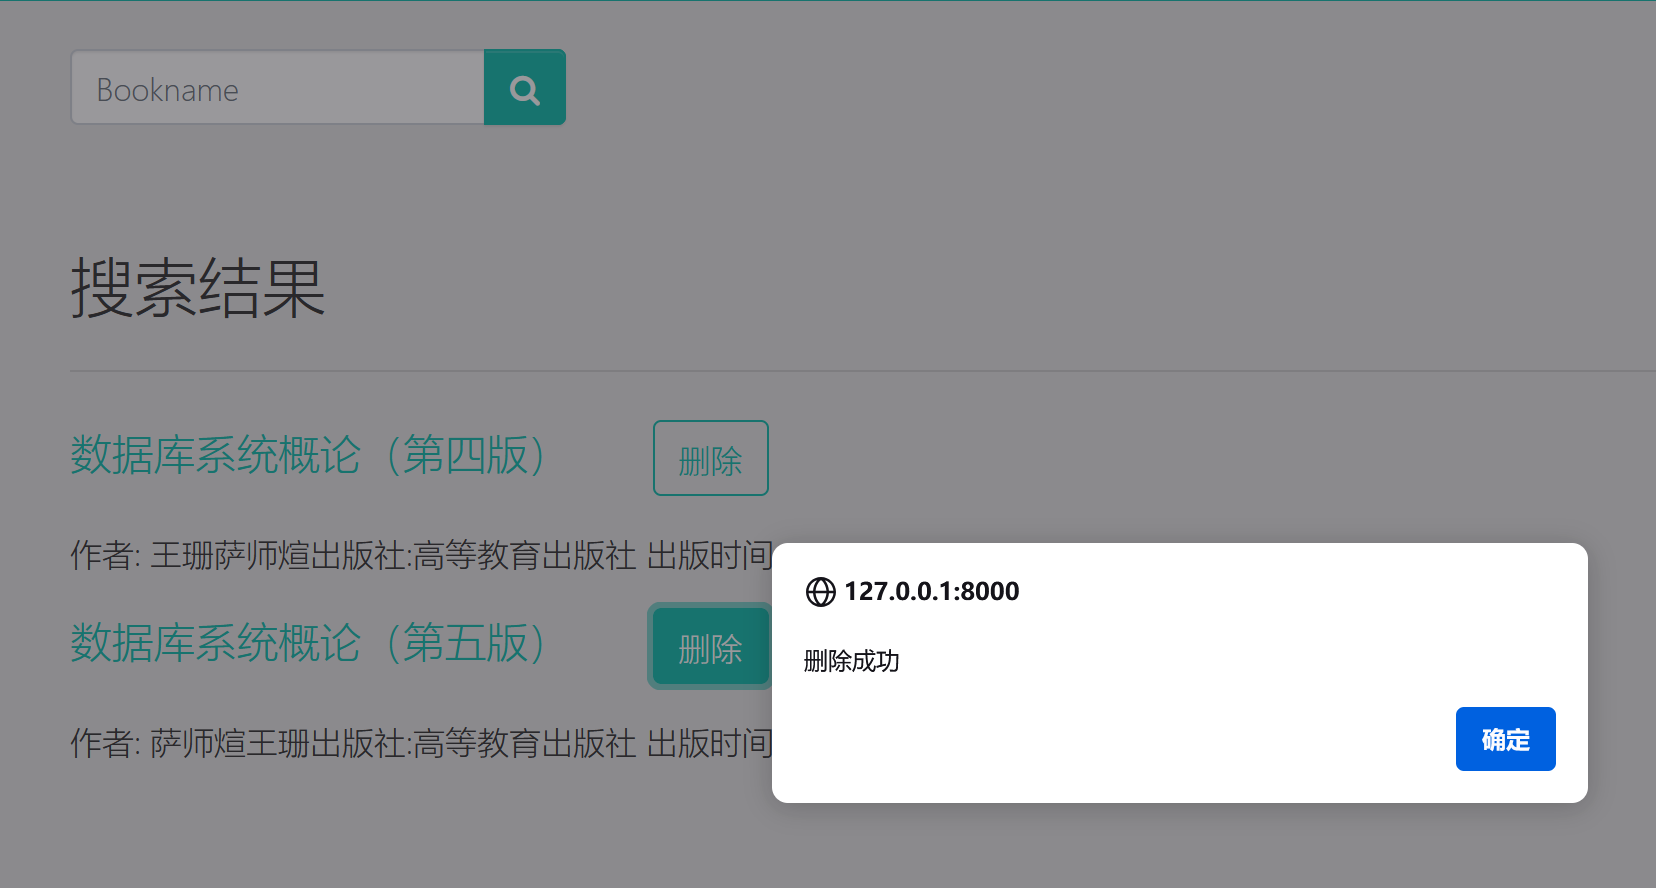
\includegraphics[width=0.7\linewidth]{images/shanchu3.png}\end{center}
\vspace{5pt}



\subsubsection{修改操作}
可以对图书信息、作者信息、馆藏信息、读者信息等进行修改操作,这里演示对读者信息修改的操作,可以修改姓名邮箱等,也可以修改密码:

\vspace{10pt}
\begin{center}
    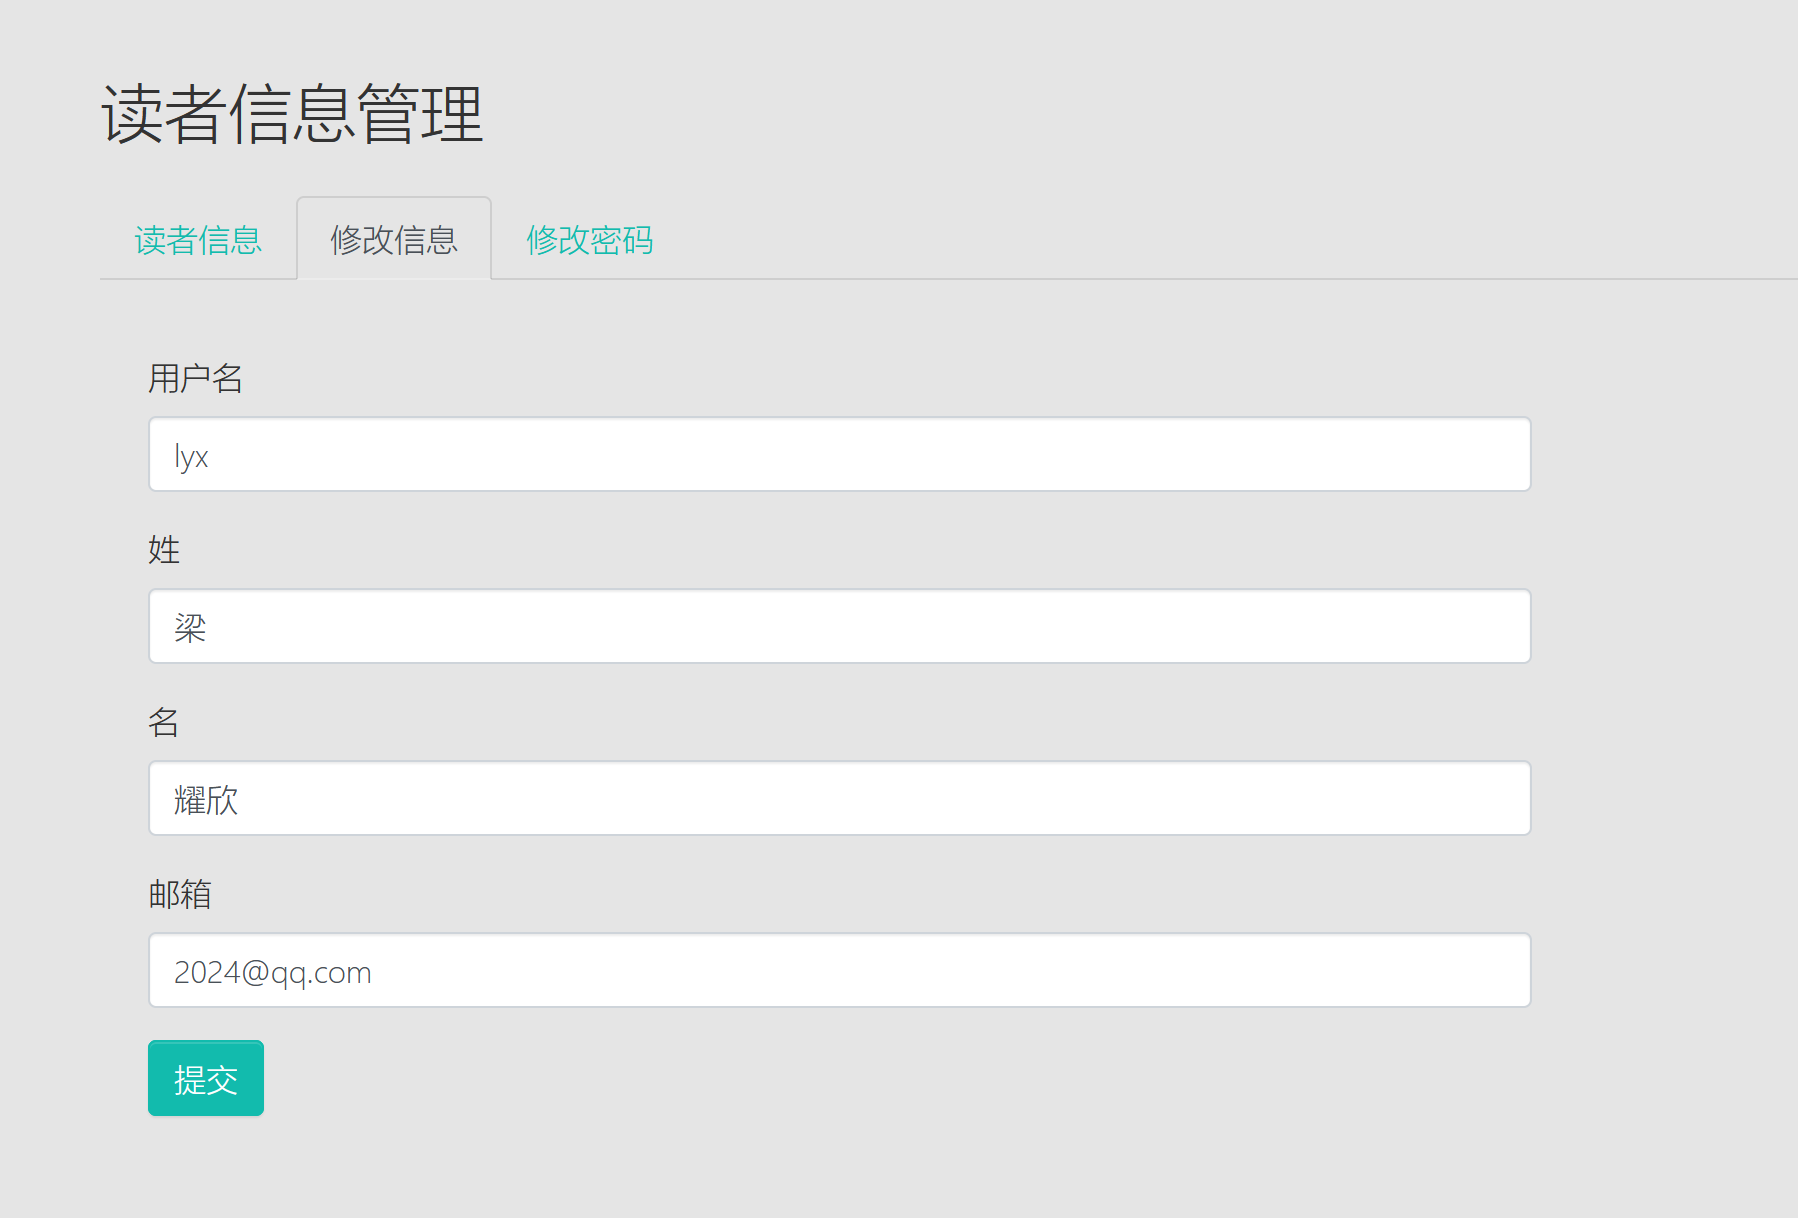
\includegraphics[width=0.7\linewidth]{images/xiugai1.png}\end{center}
\vspace{5pt}





\subsubsection{新建操作}
可以对图书信息、作者信息、馆藏信息、读者信息等进行新建操作,这里演示对书籍和读者信息新建的操作:

\vspace{10pt}
\begin{center}
    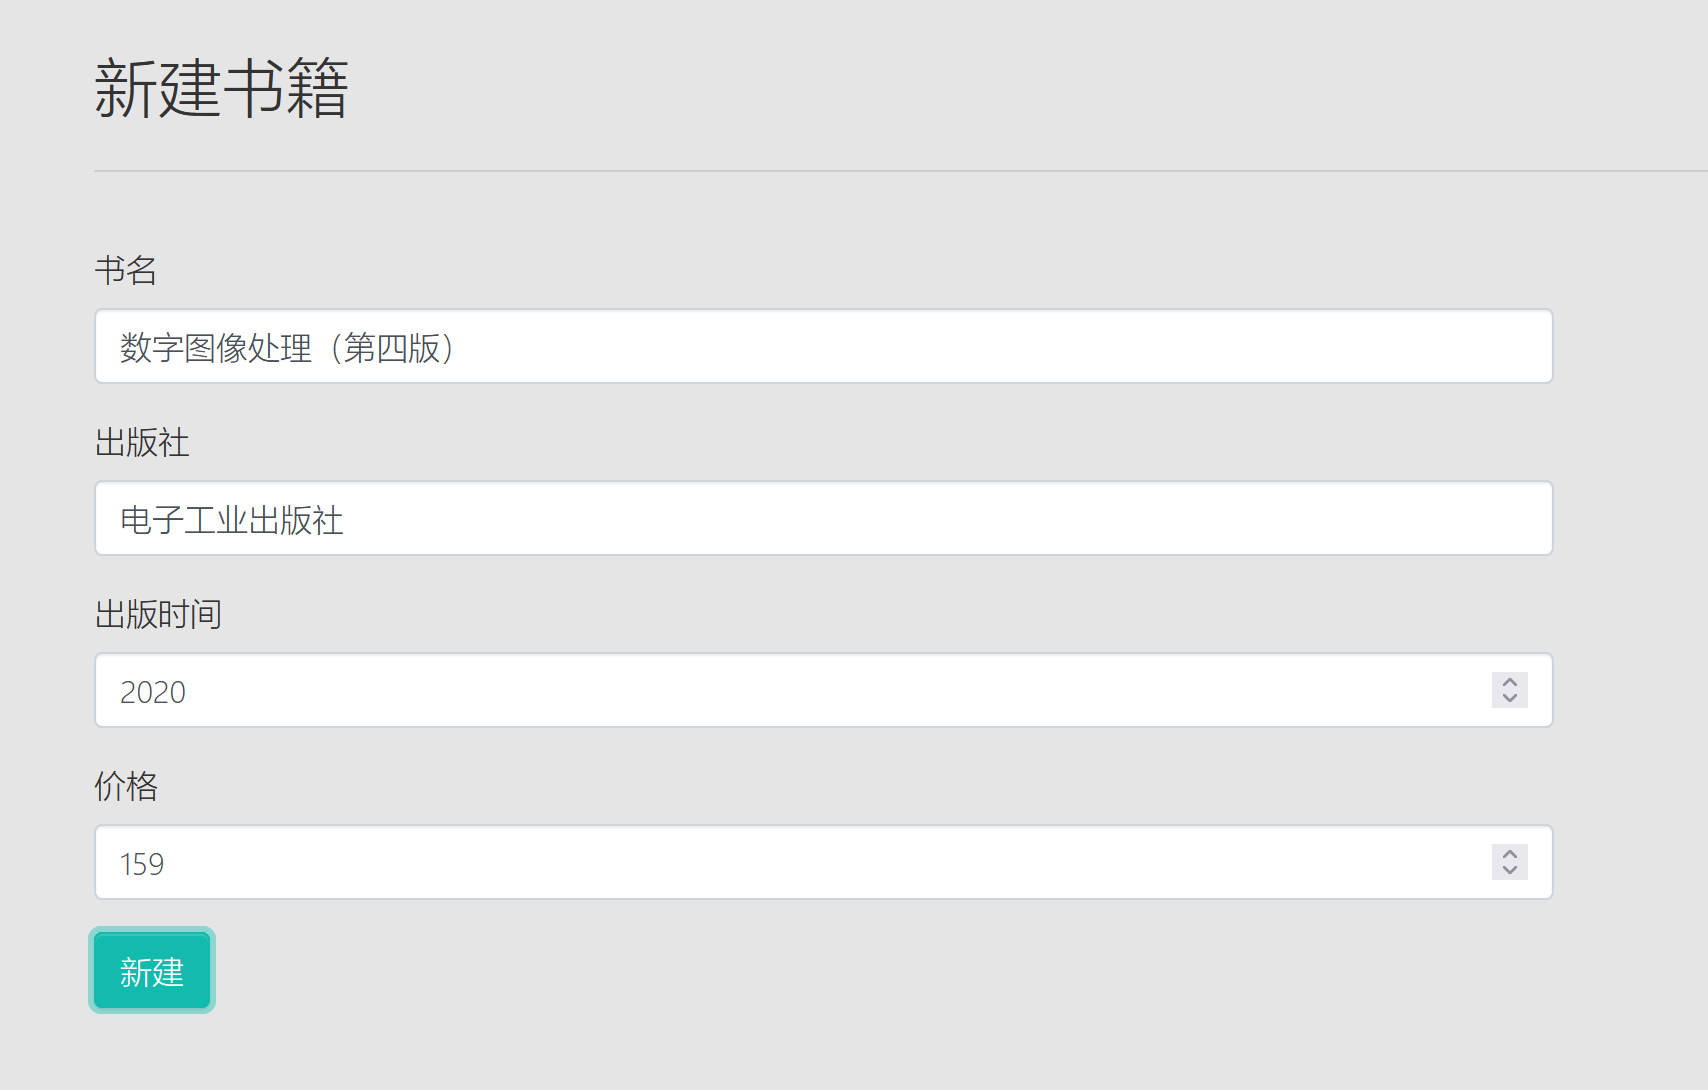
\includegraphics[width=0.7\linewidth]{images/xinjian1.png}\end{center}
\vspace{5pt}


\vspace{10pt}
\begin{center}
    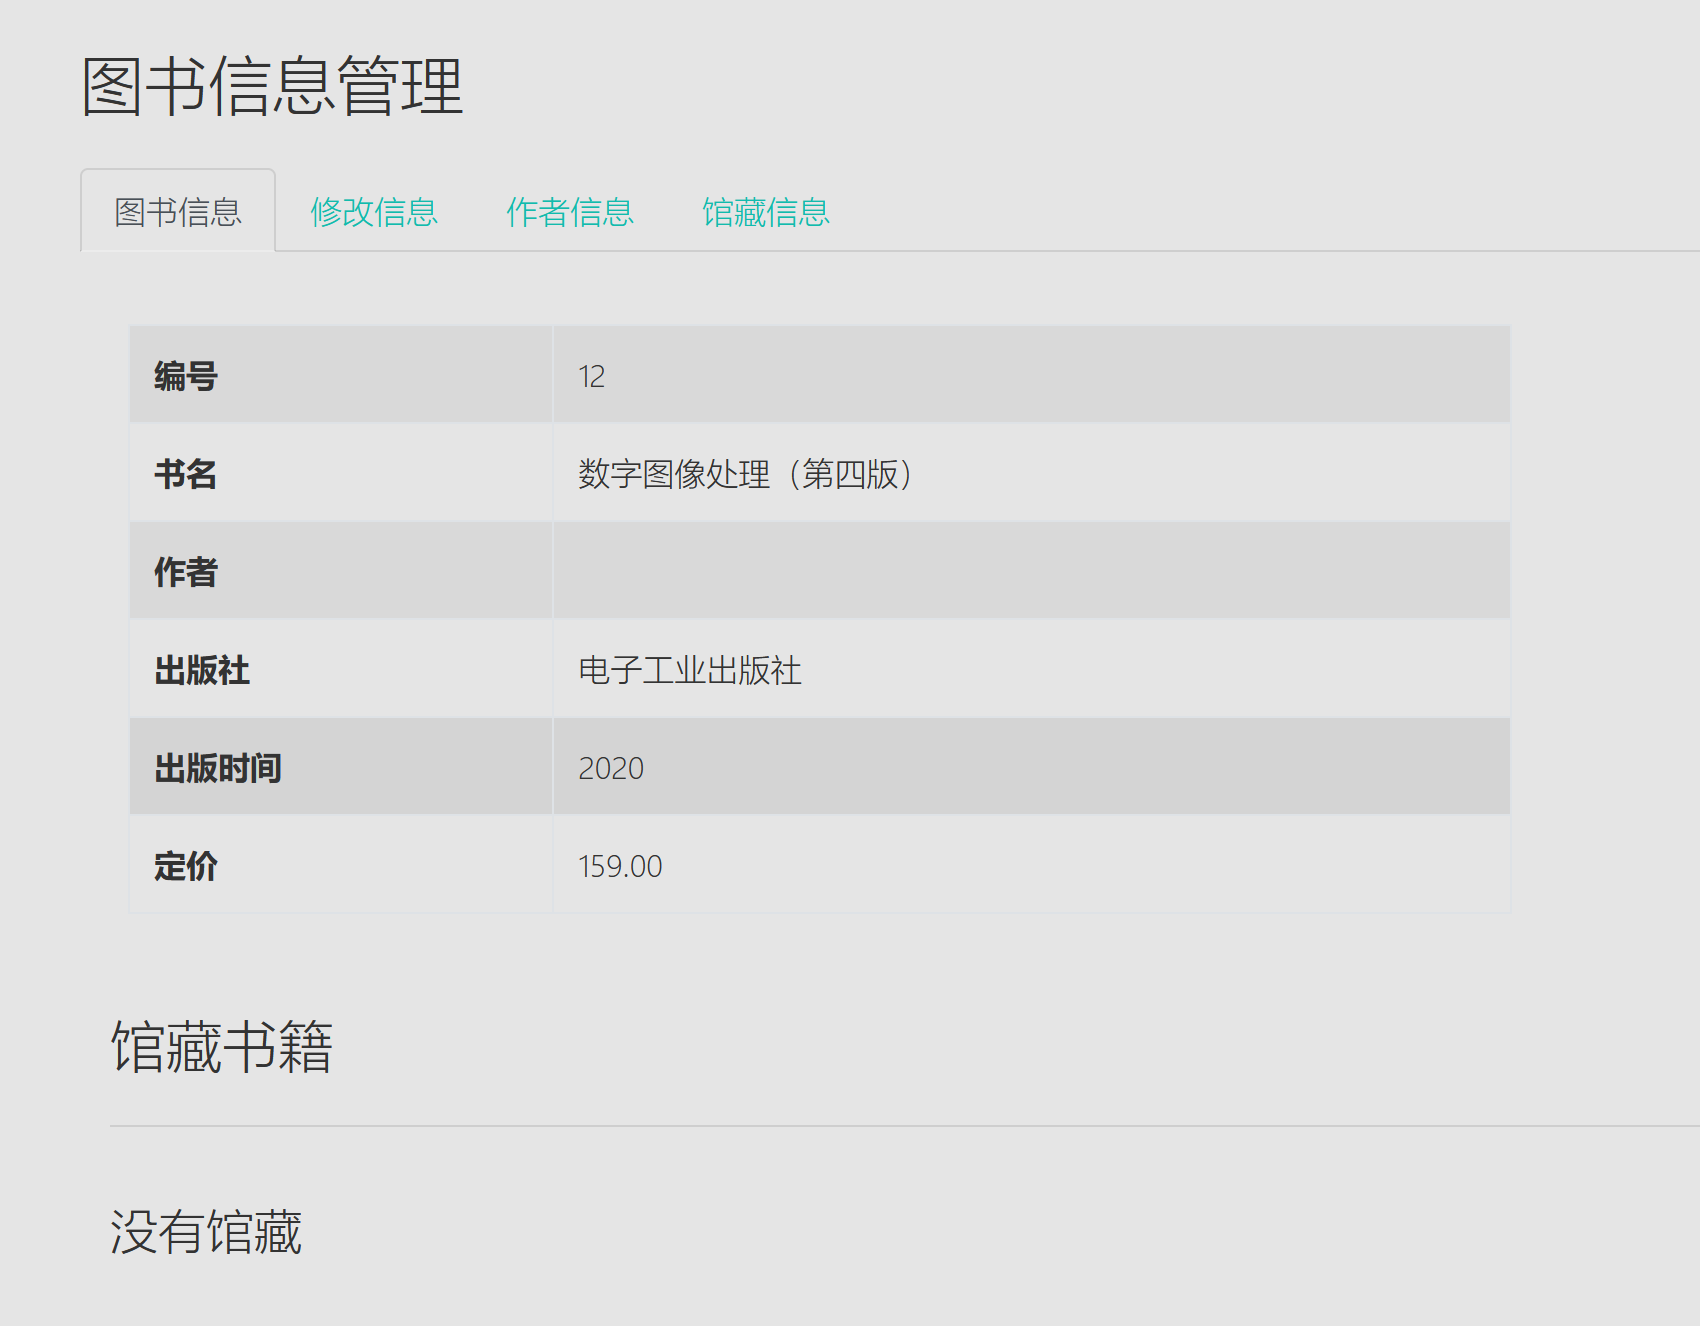
\includegraphics[width=0.7\linewidth]{images/xinjian2.png}\end{center}
\vspace{5pt}


\vspace{10pt}
\begin{center}
    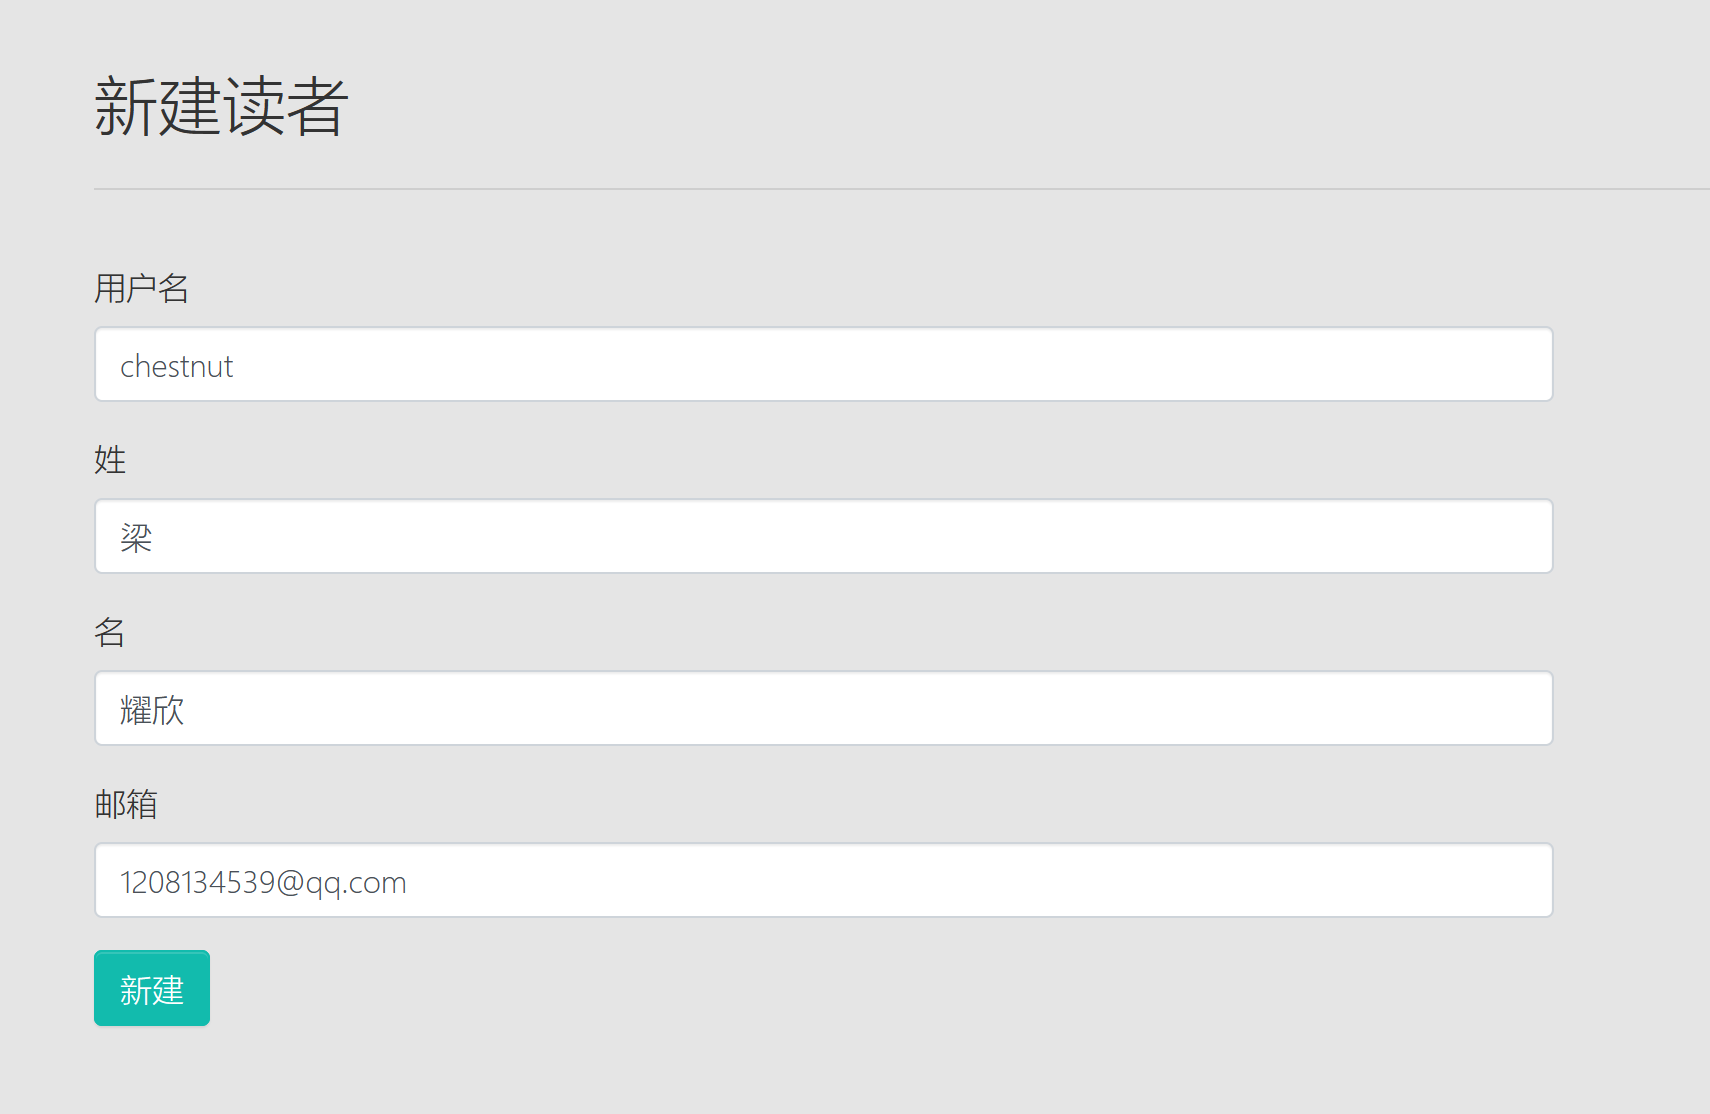
\includegraphics[width=0.7\linewidth]{images/xinjian4.png}\end{center}
\vspace{5pt}


\subsubsection{借阅操作}
在书籍在馆且读者没有罚单且读者借书不超过四本的时候,可以进行借书操作,提示信息如下:

\vspace{10pt}
\begin{center}
    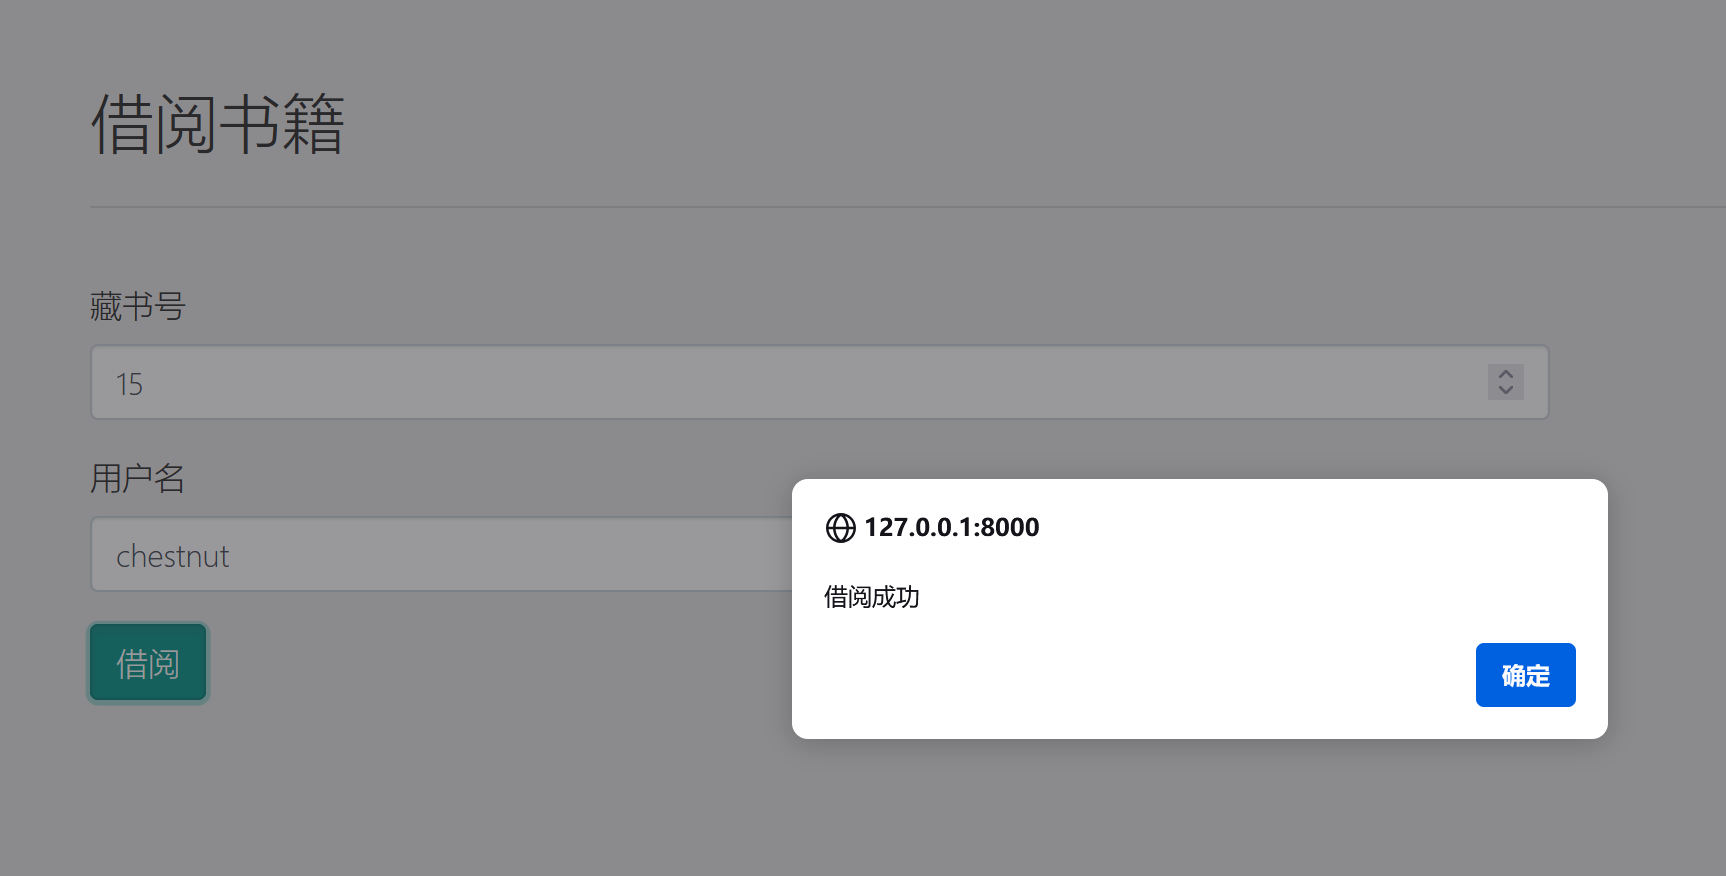
\includegraphics[width=0.7\linewidth]{images/jieyue1.png}\end{center}
\vspace{5pt}


当书籍被借走的时候提示错误信息:
\vspace{10pt}
\begin{center}
    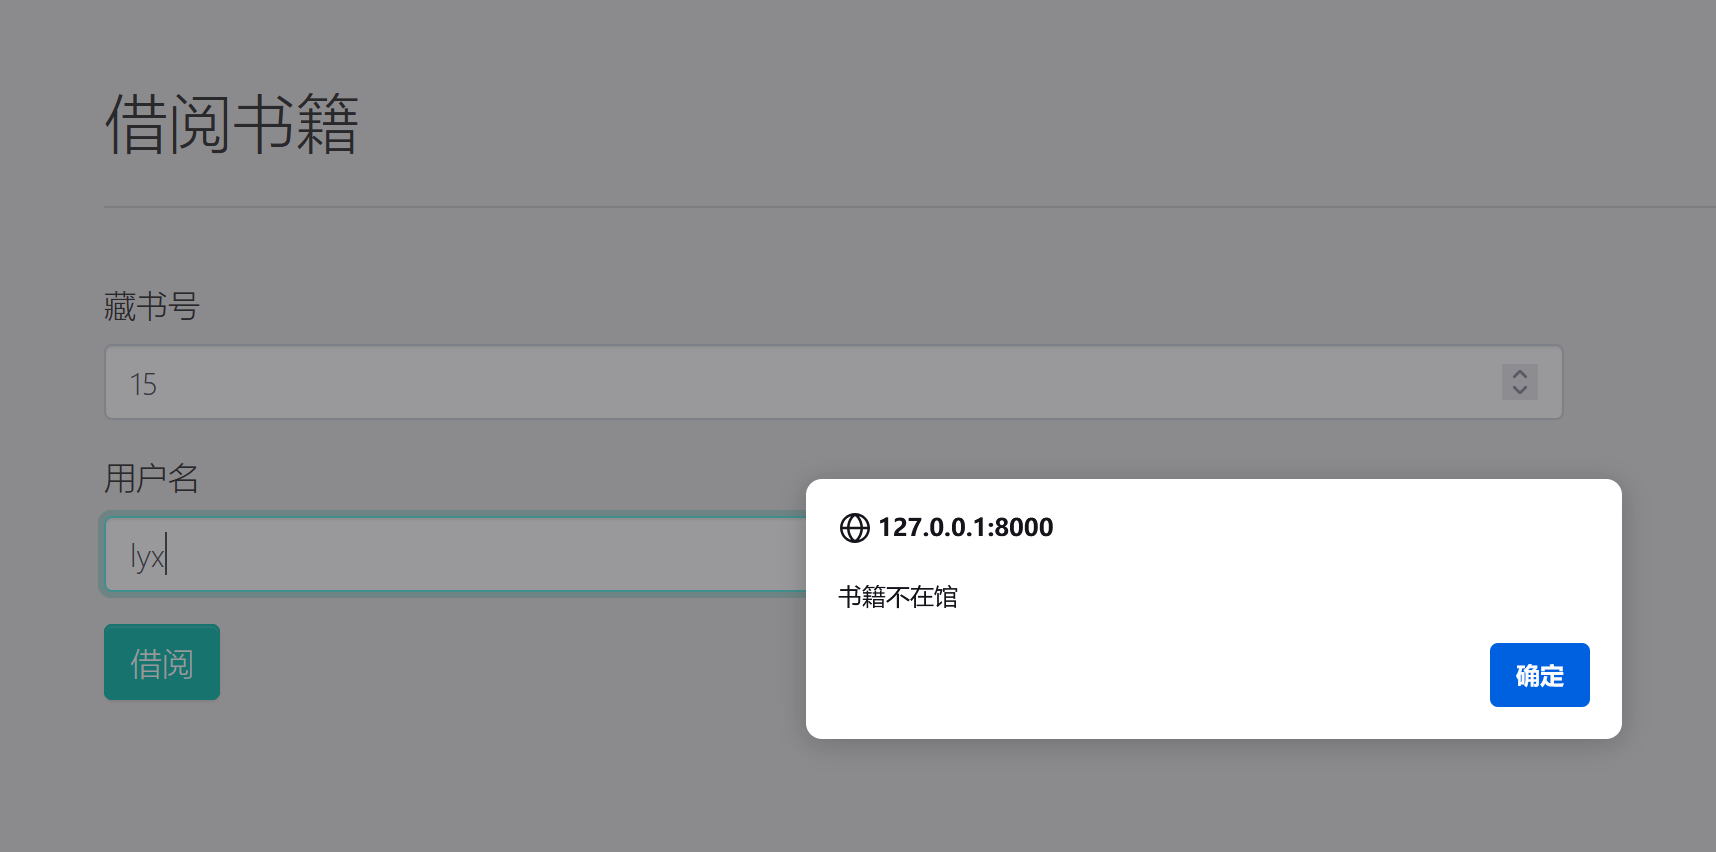
\includegraphics[width=0.7\linewidth]{images/jieyue2.png}\end{center}
\vspace{5pt}


当读者借阅有超时的时候不允许借新的书籍,需要先进行归还,这时会提示:
\vspace{10pt}
\begin{center}
    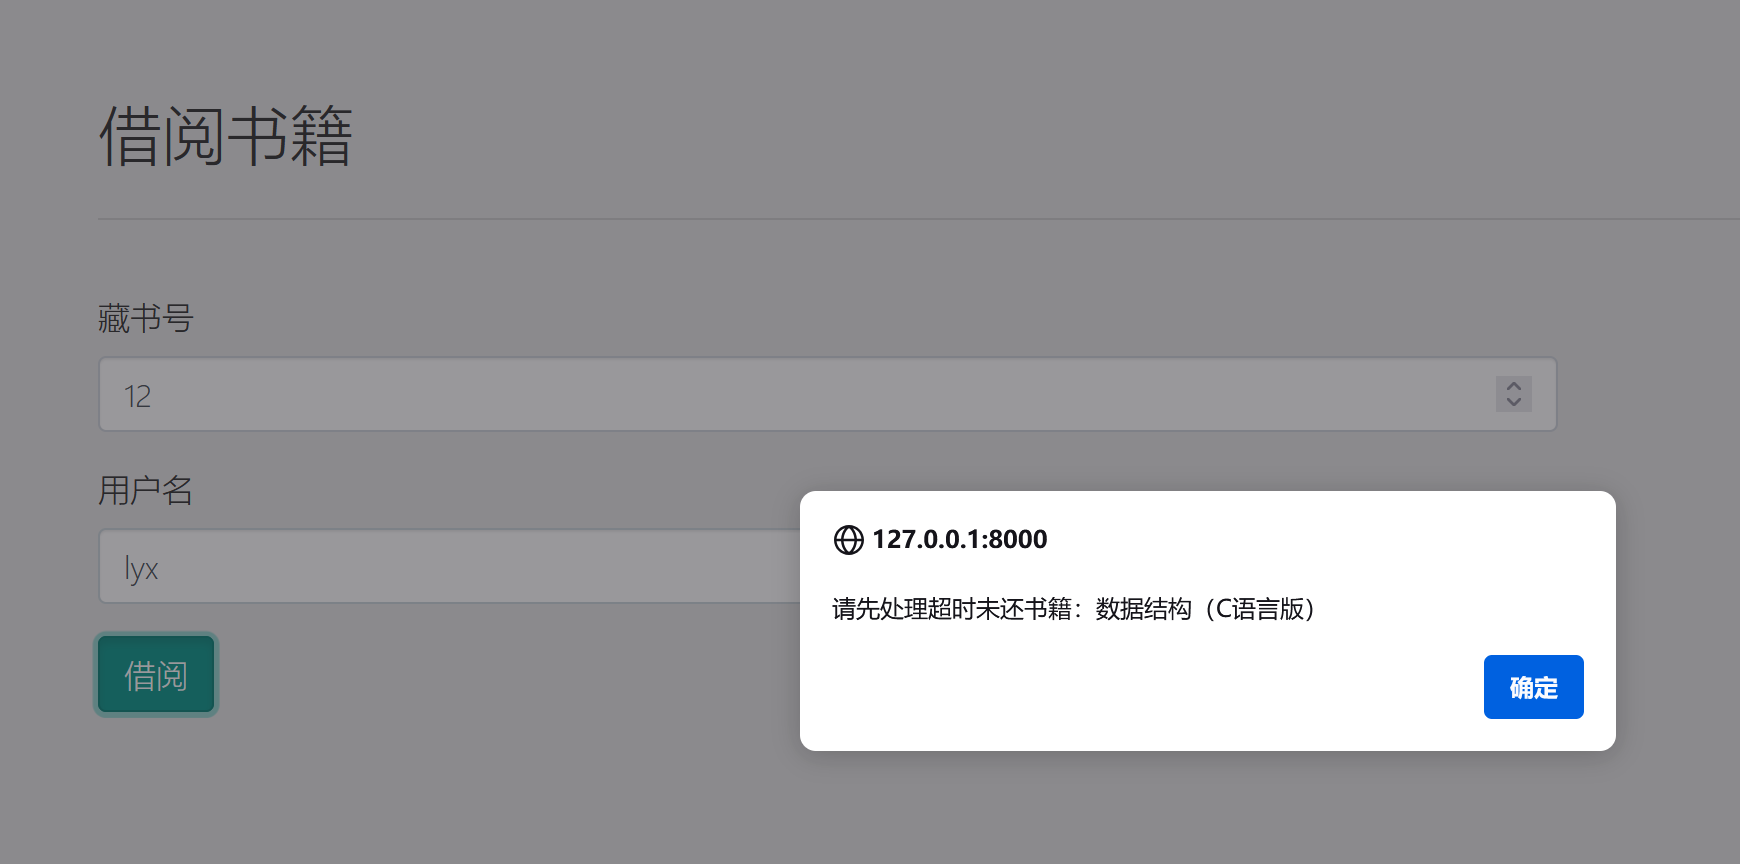
\includegraphics[width=0.7\linewidth]{images/jieyue3.png}\end{center}
\vspace{5pt}






\subsubsection{归还操作}
在管理员进行借书操作后,在归还页面输入藏书号可以进行归还操作,如果超期归还会提示生成罚单,如果书籍损坏会标记书籍,生成罚单,如果按时归还则没有提示:
\vspace{10pt}
\begin{center}
    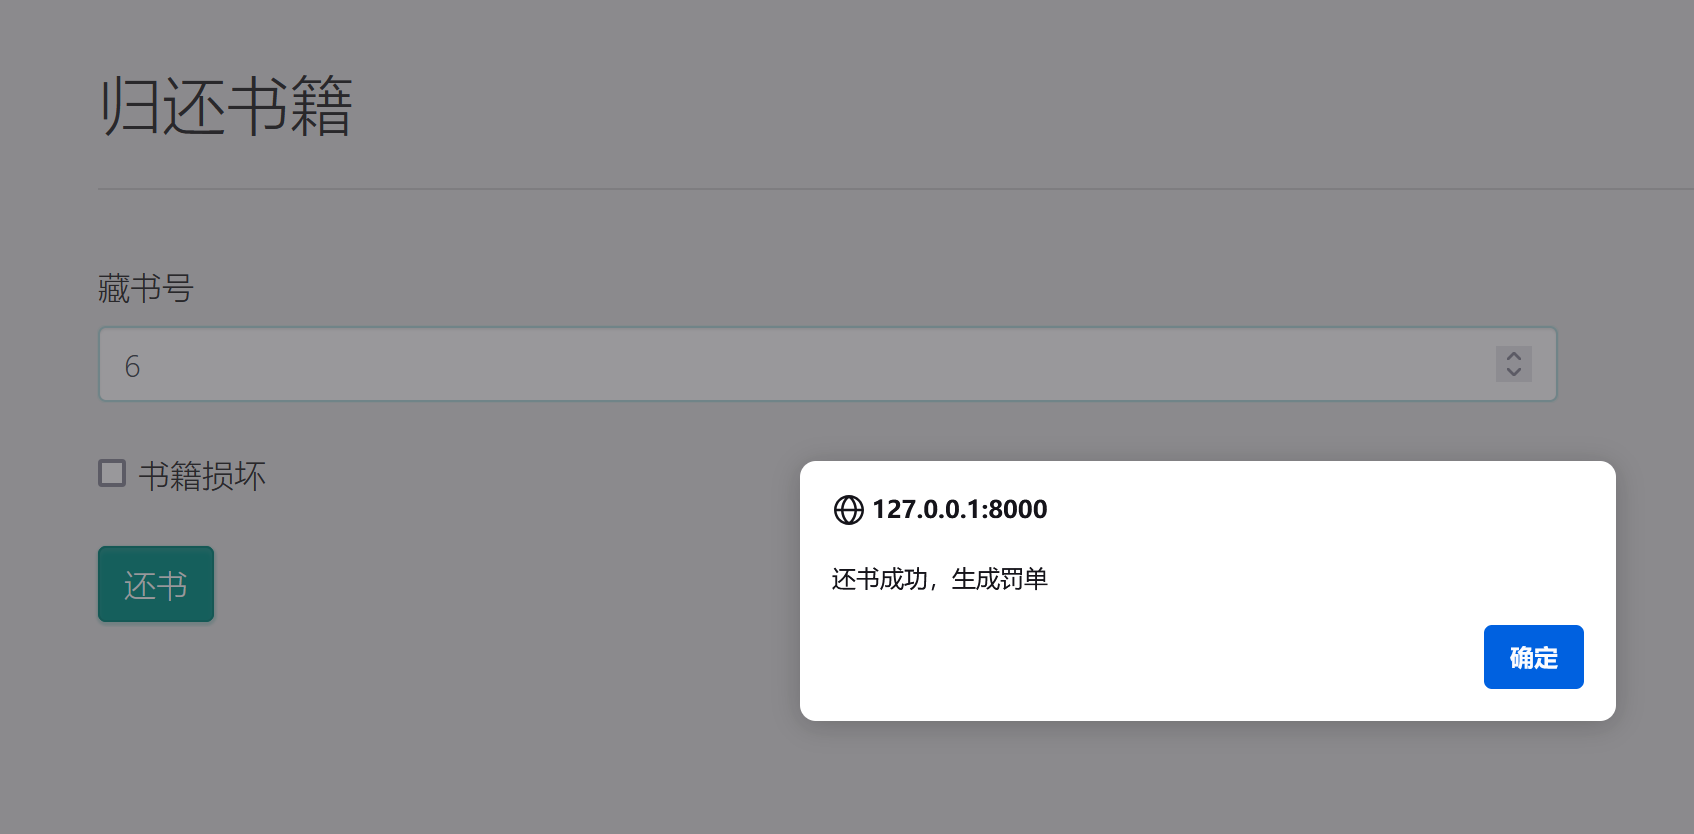
\includegraphics[width=0.7\linewidth]{images/guihuan1.png}\end{center}
\vspace{5pt}

 




\subsection{用户页面}
\subsubsection{借阅操作}
在管理员为用户借阅书籍后,用户可以在借阅记录中看到自己借阅/还书/超期的信息:

\vspace{10pt}
\begin{center}
    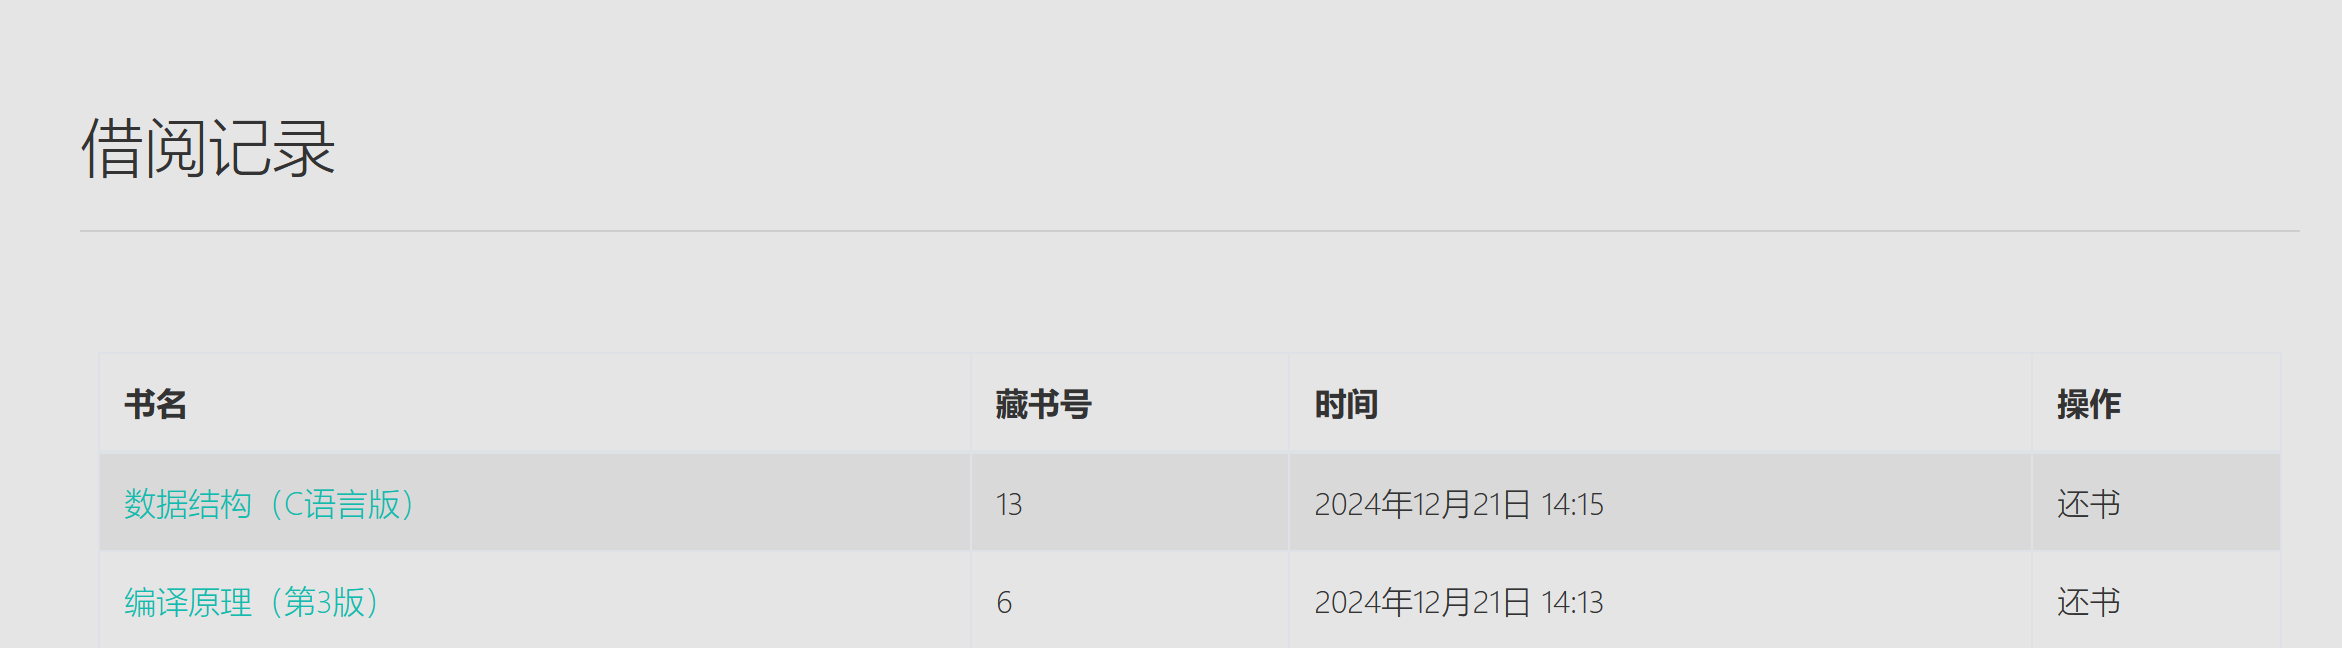
\includegraphics[width=0.7\linewidth]{images/1jieyue.png}\end{center}
\vspace{5pt}



\subsubsection{还书操作}
在待还书籍可以看到现在正在借阅的书籍,点击“续借”可以延长借书时间:

\vspace{10pt}
\begin{center}
    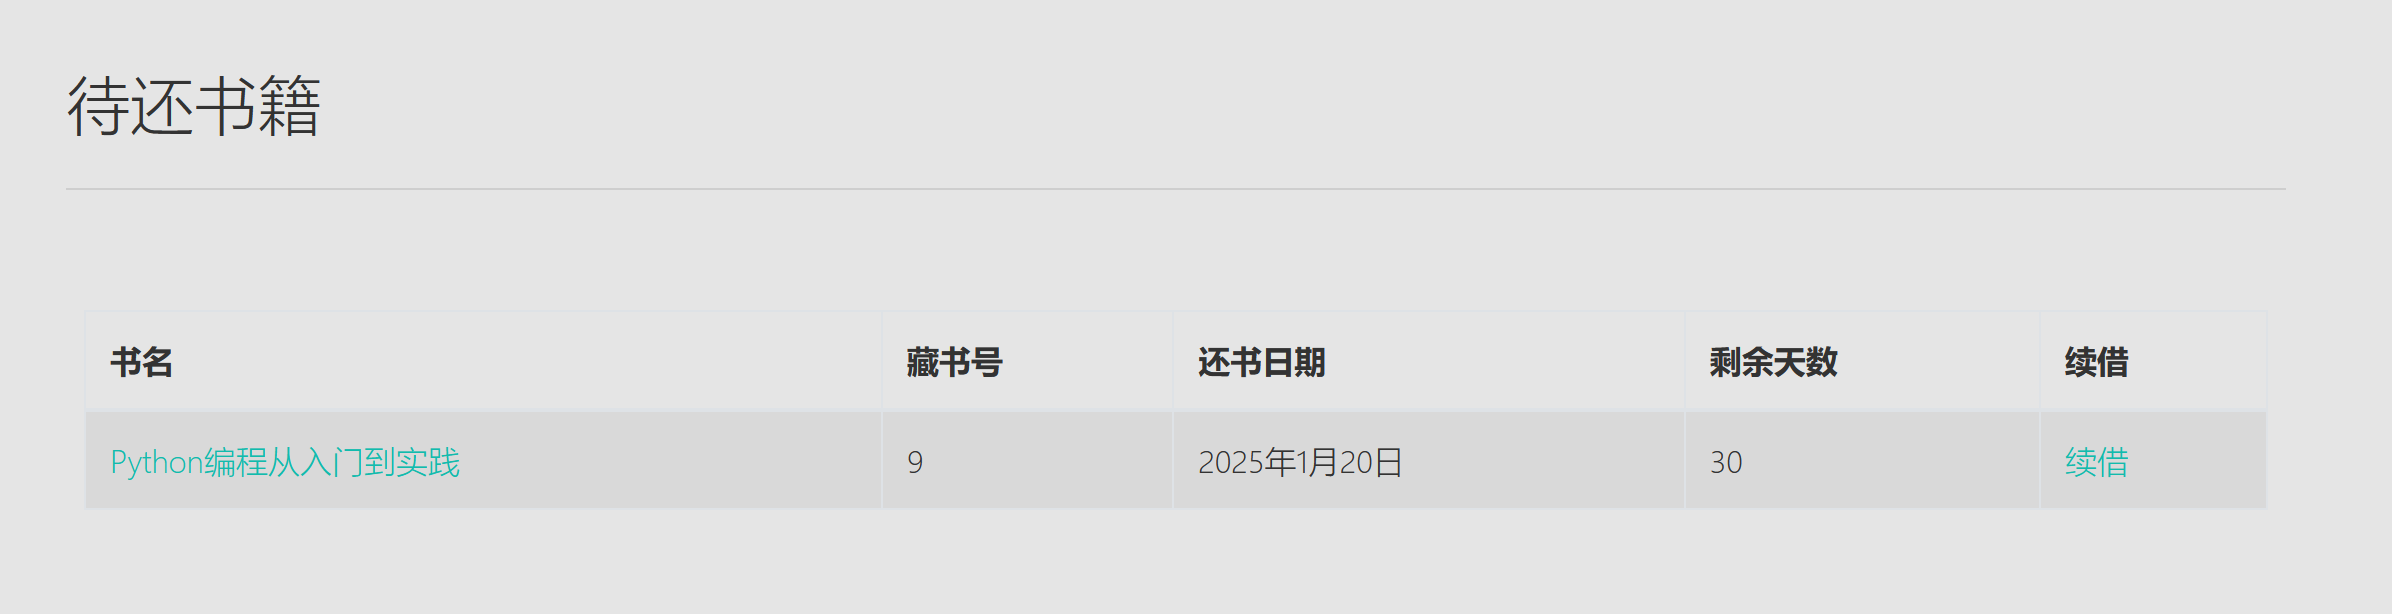
\includegraphics[width=0.7\linewidth]{images/1huanshu.png}\end{center}
\vspace{5pt}


还书成功后显示:

\vspace{10pt}
\begin{center}
    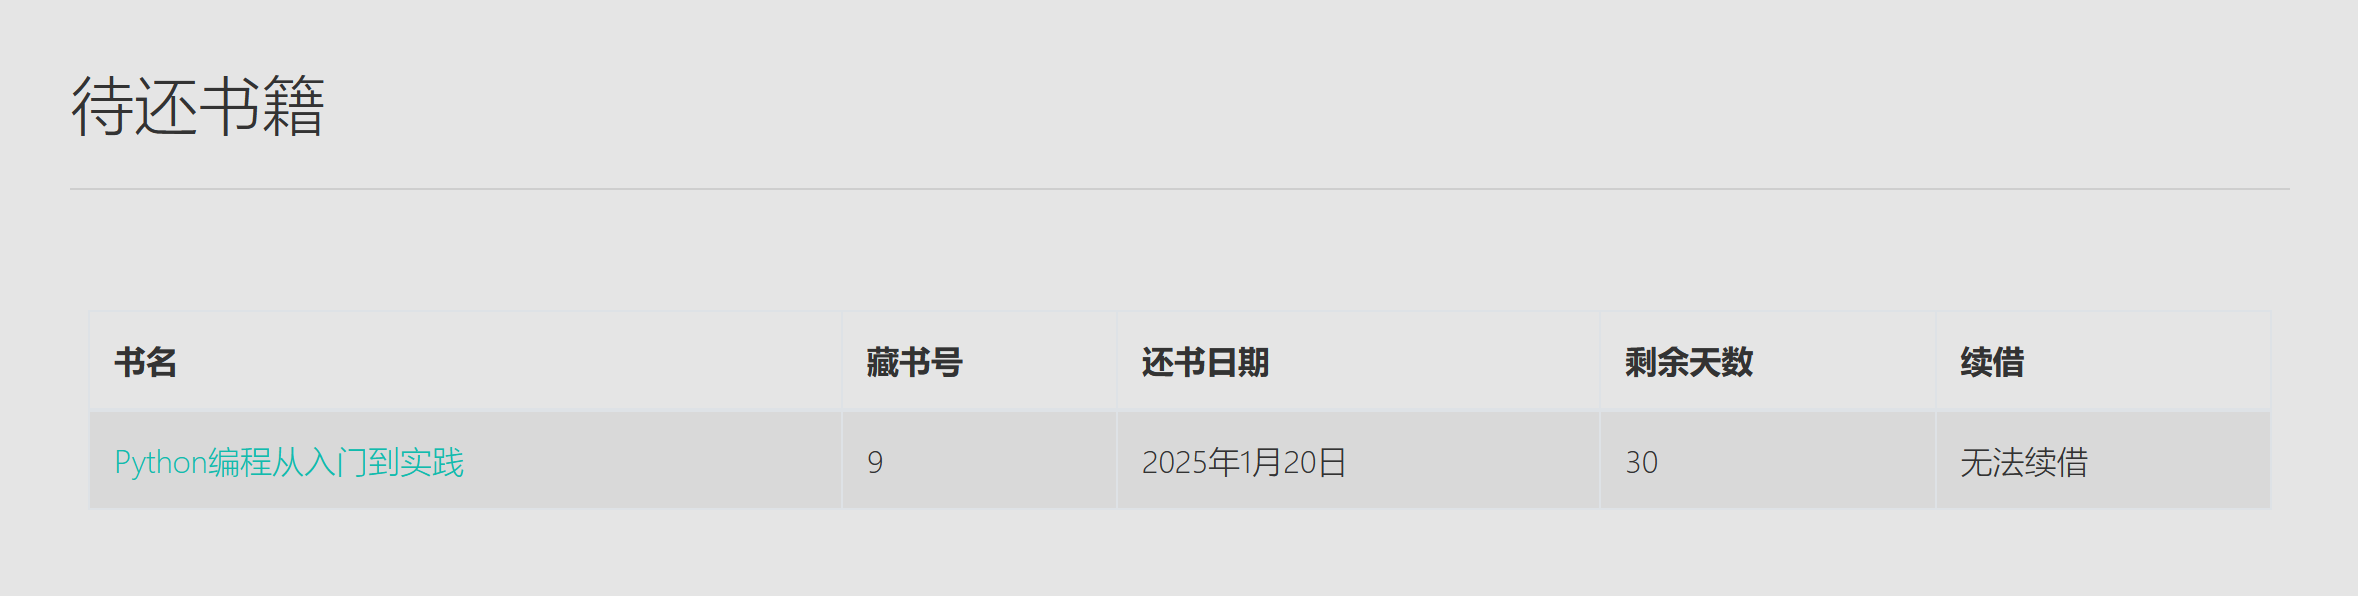
\includegraphics[width=0.7\linewidth]{images/2还书.png}\end{center}
\vspace{5pt}


\subsubsection{罚单操作}
在对图书进行归还操作后自动根据是否超期和破损产生罚单,读者可以查看自己的罚单信息并点击“待处理”进行罚单的消除,之后才可以继续借阅书籍:

\vspace{10pt}
\begin{center}
    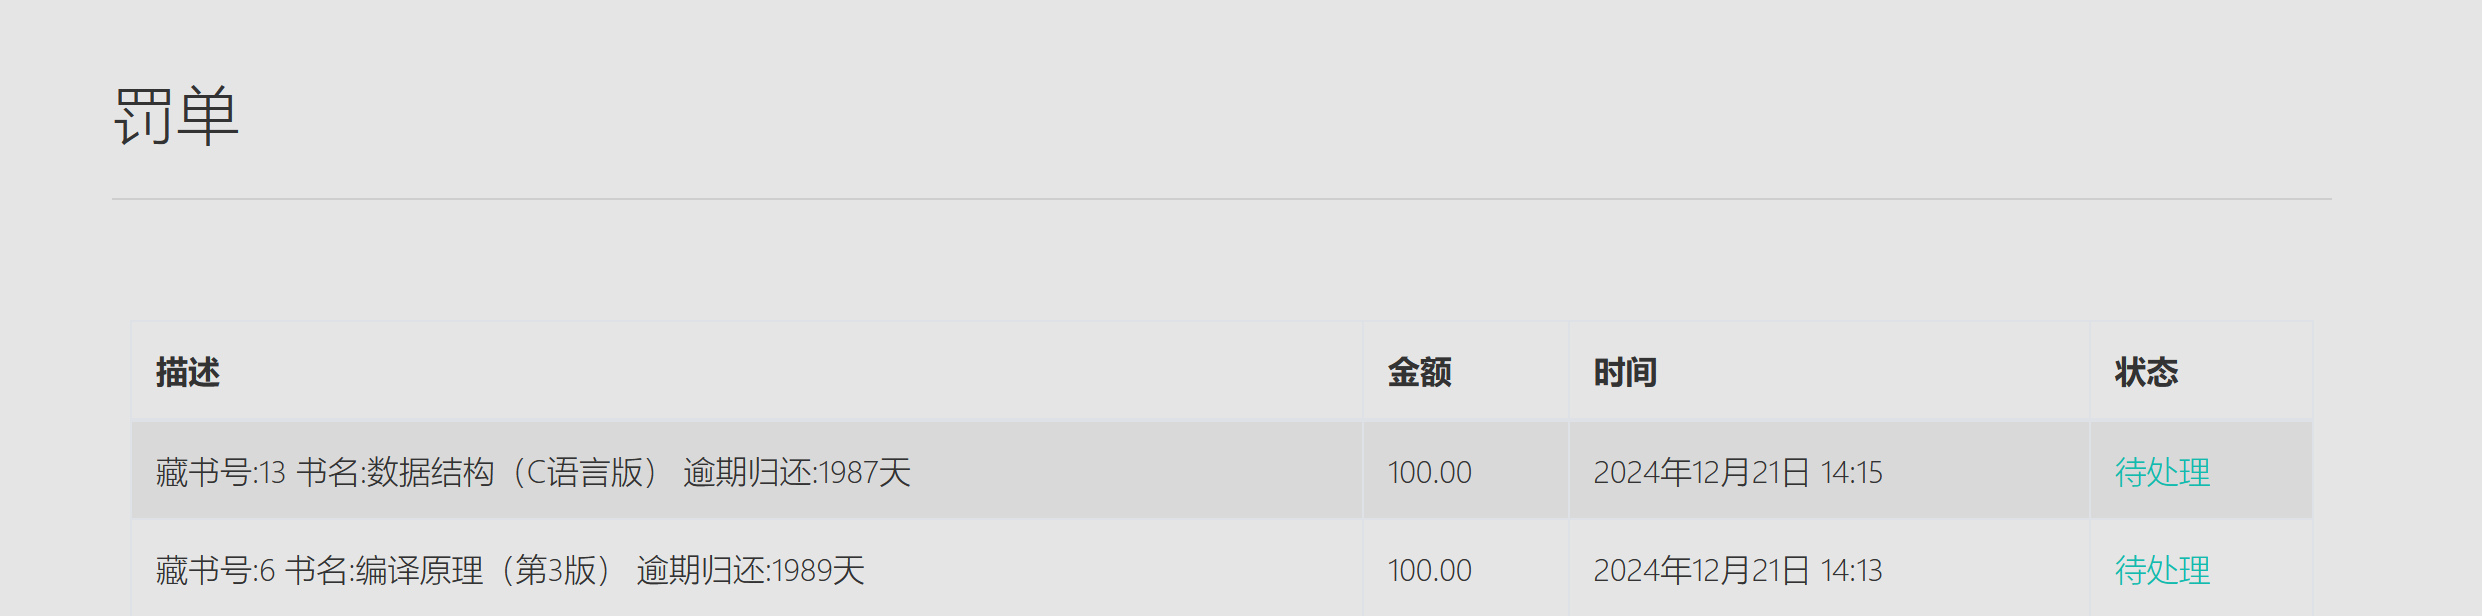
\includegraphics[width=0.7\linewidth]{images/1罚单.png}\end{center}
\vspace{5pt}


 



\section{实验总结}
这次实验的内容主要是根据暑期的实训项目修改而成,因为实训大部分时间花费在大模型的调整和接入,对数据库的应用不是很多,我加入了一些复杂的查询逻辑和判断逻辑从而更符合实验的要求。

这次实验让我收获颇丰,也让我感受到了一定的挑战。在使用SQL Server方面,我深度了解了数据库的基本操作,学会了新增用户并设置权限,掌握了SQL查询语句的多种用法以及如何实现复杂查询逻辑,这为我深入理解数据库系统奠定了坚实的基础。

在学习Python的Django框架时,我真正体会到了开发管理系统的困难与复杂。我一步步学习Django模型的基本操作、数据库迁移以及管理系统的搭建流程,熟悉了Django中的模型函数及其操作数据库的能力,这提升了我在项目开发中对数据的操作效率。我还学会了使用Django的模板系统,将业务逻辑与前端界面紧密结合,为用户提供了良好的交互体验。

在前端部分,延续暑期学校做的实训项目,我掌握了HTML和CSS的基础知识,尤其在使用Bootstrap库制作漂亮的页面界面时,我感受到视觉设计的重要性。Bootstrap让我轻松地实现了响应式布局和简洁的界面效果,极大地提升了用户的使用体验。我对JavaScript也有了一些基本了解,虽然起初感到陌生,但通过实践逐渐认识到其在前端交互中的重要性。

总体来说,这次实验让我学到了许多新的技能,也让我对自己在项目开发中的能力有了更深的认知。从数据库的设计到前端界面的实现,我经历了不少挑战,但每一次的困难都让我更加坚定。对于自己制作的成果,我感到满意,同时也意识到未来还有更多的学习和提升空间。这个过程让我收获的不仅是技术技能,更是一种对问题解决能力和实际项目开发能力的增强。

\end{document}
